\documentclass[11pt,a4paper]{article}
\usepackage[utf8]{inputenc}
\usepackage[T1]{fontenc}
\usepackage[spanish,es-tabla]{babel}
\usepackage{amsmath,amssymb}
\usepackage{graphicx}
\usepackage{booktabs}
\usepackage{float}
\usepackage{geometry}
\geometry{margin=2.3cm}
\usepackage{hyperref}
\hypersetup{colorlinks=true, linkcolor=blue, urlcolor=blue, citecolor=blue}

\title{\textbf{Informe Completo de Prácticas de Laboratorio: Estudio Integral de la Corrosión}\\[0.4em]\large Análisis Experimental de Factores Ambientales, Mecánicos, Inhibidores y Protección Electroquímica}
\author{\textbf{Resistencia de Materiales y Diseño Mecánico (RMDM)}\\4º Grado en Ingeniería Química -- Curso 2026/2027}
\date{\today}

\begin{document}

\maketitle

\begin{abstract}
El presente informe recoge el tratamiento cuantitativo riguroso, análisis electroquímico, representación gráfica y conclusiones de la totalidad de las sesiones prácticas de corrosión (Experimentos 3.1 a 3.6). Se evalúa el efecto del pH inicial en electrodos de Zinc y Cobre mediante diagramas de Pourbaix (con gráficas conjuntas e individuales), la aceleración corrosiva generada por concentración de esfuerzos mecánicos y acritud en probetas de acero, la influencia de la presencia y transporte de oxígeno disuelto en medio salino, la cinética de inhibición pasivante por adición de fosfato trisódico ($\text{Na}_3\text{PO}_4$) calculada por incrementos temporales, el mecanismo de protección catódica por corriente impresa en medio alcalino y, finalmente, el comportamiento de pares galvánicos bimetálicos ($\text{Acero}-\text{Zn}$ y $\text{Acero}-\text{Cu}$).
\end{abstract}

\tableofcontents
\newpage

% =============================================================================
\section{Introducción y Objetivos Generales}
% =============================================================================
La corrosión metálica constituye un proceso electroquímico espontáneo y destructivo en el que los metales retornan a estados termodinámicamente más estables (óxidos, hidróxidos o sales). Los objetivos fundamentales de estas prácticas son:
\begin{enumerate}
    \item Identificar en los \textbf{Diagramas de Pourbaix} ($E-\text{pH}$) las zonas de inmunidad, corrosión activa y pasivación de metales de interés en ingeniería ($\text{Fe}$, $\text{Zn}$, $\text{Cu}$).
    \item Cuantificar la influencia de variables operacionales críticas: pH, solicitaciones mecánicas residuales, disponibilidad de despolarizantes catódicos ($\text{O}_2$) y presencia de inhibidores químicos.
    \item Calcular las velocidades de corrosión de forma puntual/incremental entre pesadas consecutivas:
    \begin{equation}
        v_i = \frac{-(m_i - m_{i-1})\cdot 1000}{t_i - t_{i-1}} \quad [\text{mg/h}]
    \end{equation}
    \item Evaluar métodos industriales de prevención y control: pasivación por inhibidores anódicos, protección catódica por corriente impresa y análisis de compatibilidad en acoplamientos galvánicos.
\end{enumerate}

% =============================================================================
\section{Experimento 3.1: Efecto del pH en la Velocidad de Corrosión}
% =============================================================================
\subsection{Fundamento y Reacciones Químicas}
Se analiza el comportamiento de electrodos de Zinc ($\text{Zn}$) y Cobre ($\text{Cu}$) sumergidos en agua aireada a $\text{pH}_0 = 4$ y $\text{pH}_0 = 9$.

\subsubsection{Electrodo de Zinc ($\text{Zn}$)}
\begin{itemize}
    \item \textbf{Medio Ácido ($\text{pH}_0 = 4$)}: El potencial estándar del par $\text{Zn}^{2+}/\text{Zn}$ es marcadamente negativo ($E^0 = -0.763\text{ V}$), encontrándose en la \textbf{zona de corrosión activa}:
    \begin{align}
        \text{Semirreacción anódica:} \quad & \text{Zn(s)} \longrightarrow \text{Zn}^{2+}(\text{aq}) + 2e^- \\
        \text{Semirreacción catódica:} \quad & 2\text{H}^+ + 2e^- \longrightarrow \text{H}_2(\text{g}) \quad \text{y} \quad \text{O}_2 + 4\text{H}^+ + 4e^- \longrightarrow 2\text{H}_2\text{O}
    \end{align}
    El consumo de protones $\text{H}^+$ desplaza el pH experimental desde $4.10$ hasta $6.86$.
    \item \textbf{Medio Básico ($\text{pH}_0 = 9$)}: El zinc penetra en su \textbf{zona de pasivación}, formando hidróxido de zinc insoluble:
    \begin{equation}
        \text{Zn}^{2+} + 2\text{OH}^- \longrightarrow \text{Zn(OH)}_2(\text{s}) \quad \text{o} \quad \text{ZnO}\cdot\text{H}_2\text{O}
    \end{equation}
    Esta película adherente actúa como barrera difusional, reduciendo la velocidad de corrosión drásticamente frente al medio ácido.
\end{itemize}

\subsubsection{Electrodo de Cobre ($\text{Cu}$)}
El cobre tiene un potencial estándar noble ($E^0_{\text{Cu}^{2+}/\text{Cu}} = +0.34\text{ V}$). No es atacado por ácidos no oxidantes en ausencia de oxígeno:
\begin{align}
    \text{Semirreacción anódica:} \quad & \text{Cu(s)} \longrightarrow \text{Cu}^{2+}(\text{aq}) + 2e^- \\
    \text{Semirreacción catódica:} \quad & \text{O}_2 + 2\text{H}_2\text{O} + 4e^- \longrightarrow 4\text{OH}^- \quad (E^0 = +0.401\text{ V})
\end{align}
A pH 4 la velocidad es muy baja y a pH 9 es casi nula por formación de óxidos pasivos $\text{Cu}_2\text{O}/\text{CuO}$.

\subsection{Resultados Experimentales y Tablas}
\begin{table}[H]
\centering
\caption{Zinc en agua aireada -- $\text{pH}_{\text{inicial}} = 4$}
\label{tab:3_1_zn_ph4}
\begin{tabular}{ccccccc}
\toprule
t (días) & t (h) & Masa (g) & Masa (\%) & Pérdida (mg) & Velocidad (mg/h) & pH \\
\midrule
0.0000 & 0.0000 & 7.7700 & 100.00 & 0.0000 & 0.0000 & 4.1000 \\
0.9380 & 22.5100 & 7.7332 & 99.5264 & 36.8000 & 1.6347 & 4.6700 \\
1.9480 & 46.7500 & 7.6889 & 98.9562 & 81.1000 & 1.8276 & 5.2200 \\
2.9480 & 70.7500 & 7.6482 & 98.4324 & 121.80 & 1.6958 & 5.6300 \\
5.8650 & 140.76 & 7.6098 & 97.9382 & 160.20 & 0.5485 & 6.5800 \\
6.0750 & 145.80 & 7.6077 & 97.9112 & 162.30 & 0.4167 & 6.8600 \\
\bottomrule
\end{tabular}
\end{table}

\begin{table}[H]
\centering
\caption{Zinc en agua aireada -- $\text{pH}_{\text{inicial}} = 9$}
\label{tab:3_1_zn_ph9}
\begin{tabular}{ccccccc}
\toprule
t (días) & t (h) & Masa (g) & Masa (\%) & Pérdida (mg) & Velocidad (mg/h) & pH \\
\midrule
0.0000 & 0.0000 & 8.3209 & 100.00 & 0.0000 & 0.0000 & 9.1900 \\
0.9380 & 22.5100 & 8.3147 & 99.9255 & 6.2000 & 0.2754 & 9.1500 \\
1.9480 & 46.7500 & 8.3116 & 99.8882 & 9.3000 & 0.1279 & 9.5400 \\
2.9480 & 70.7500 & 8.3082 & 99.8474 & 12.7000 & 0.1417 & 9.3400 \\
5.8650 & 140.76 & 8.3013 & 99.7644 & 19.6000 & 0.0986 & 9.4000 \\
6.0750 & 145.80 & 8.2997 & 99.7452 & 21.2000 & 0.3175 & 9.6000 \\
\bottomrule
\end{tabular}
\end{table}

\begin{table}[H]
\centering
\caption{Cobre en agua aireada -- $\text{pH}_{\text{inicial}} = 4$}
\label{tab:3_1_cu_ph4}
\begin{tabular}{ccccccc}
\toprule
t (días) & t (h) & Masa (g) & Masa (\%) & Pérdida (mg) & Velocidad (mg/h) & pH \\
\midrule
0.0000 & 0.0000 & 9.6686 & 100.00 & 0.0000 & 0.0000 & 4.0900 \\
0.9380 & 22.5100 & 9.6583 & 99.8935 & 10.3000 & 0.4575 & 4.1200 \\
1.9480 & 46.7500 & 9.6584 & 99.8945 & 10.2000 & -0.0041 & 4.4300 \\
2.9480 & 70.7500 & 9.6574 & 99.8842 & 11.2000 & 0.0417 & 4.3500 \\
5.8650 & 140.76 & 9.6554 & 99.8635 & 13.2000 & 0.0286 & 4.3800 \\
6.0750 & 145.80 & 9.6548 & 99.8573 & 13.8000 & 0.1190 & 4.3800 \\
\bottomrule
\end{tabular}
\end{table}

\begin{table}[H]
\centering
\caption{Cobre en agua aireada -- $\text{pH}_{\text{inicial}} = 9$}
\label{tab:3_1_cu_ph9}
\begin{tabular}{ccccccc}
\toprule
t (días) & t (h) & Masa (g) & Masa (\%) & Pérdida (mg) & Velocidad (mg/h) & pH \\
\midrule
0.0000 & 0.0000 & 9.7060 & 100.00 & 0.0000 & 0.0000 & 9.1700 \\
0.9380 & 22.5100 & 9.7048 & 99.9876 & 1.2000 & 0.0533 & 9.1200 \\
1.9480 & 46.7500 & 9.7046 & 99.9856 & 1.4000 & 0.0083 & 9.5200 \\
2.9480 & 70.7500 & 9.7046 & 99.9856 & 1.4000 & -0.0000 & 9.5400 \\
5.8650 & 140.76 & 9.7024 & 99.9629 & 3.6000 & 0.0314 & 9.3400 \\
6.0750 & 145.80 & 9.7020 & 99.9588 & 4.0000 & 0.0794 & - \\
\bottomrule
\end{tabular}
\end{table}


\subsection{Representación Gráfica (Conjunta e Individual)}

\begin{figure}[H]
    \centering
    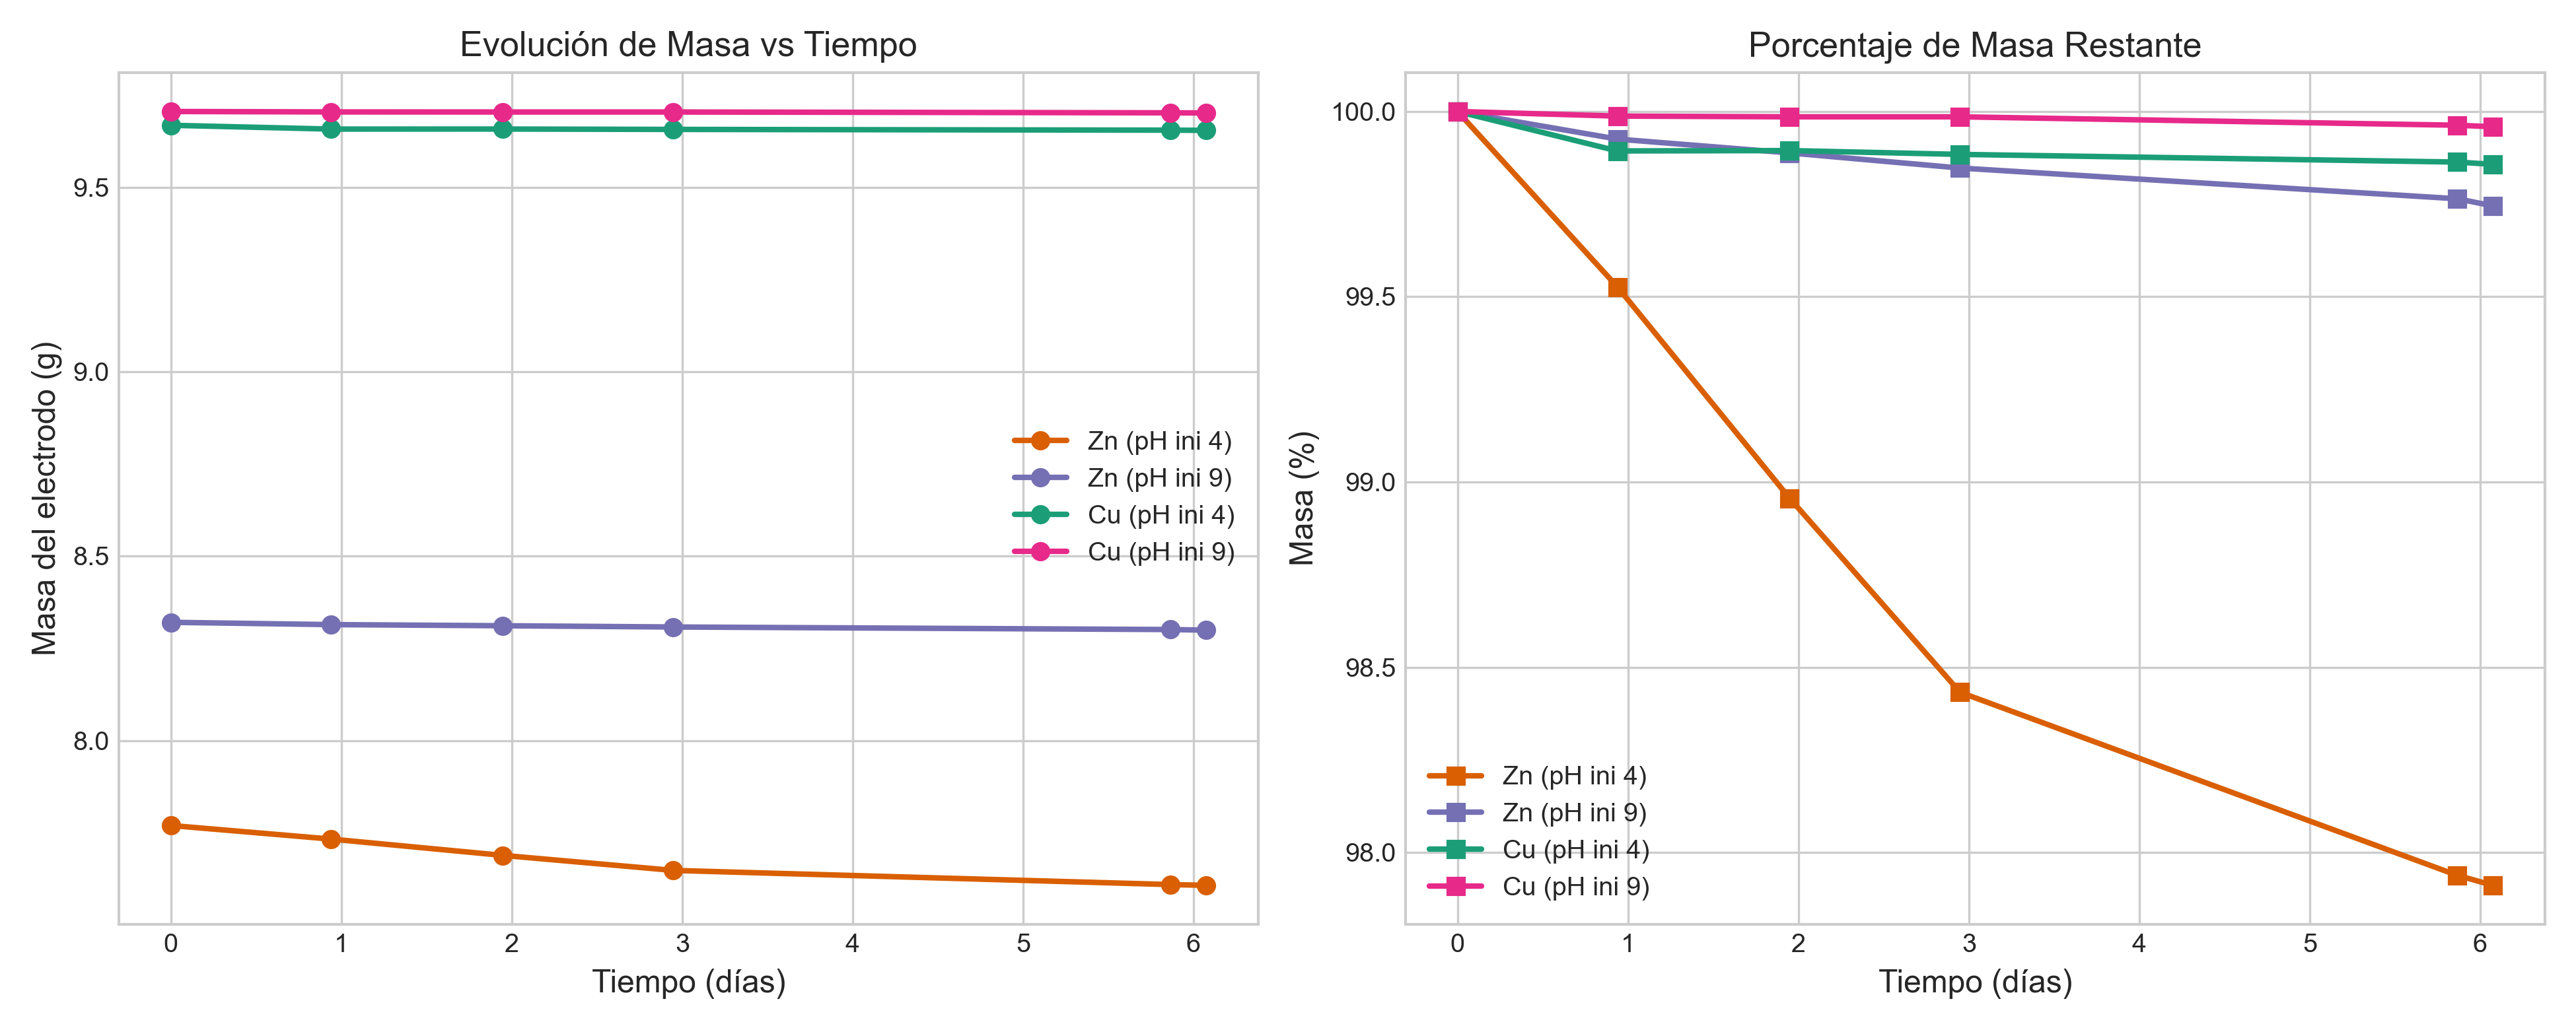
\includegraphics[width=0.92\textwidth]{resultados_practica_corrosion/exp_3_1_conjunto_masa_y_pct.png}
    \caption{Evolución conjunta de la masa absoluta (g) y del porcentaje restante (\%) para electrodos de Zn y Cu.}
    \label{fig:exp_3_1_masa_pct}
\end{figure}

\begin{figure}[H]
    \centering
    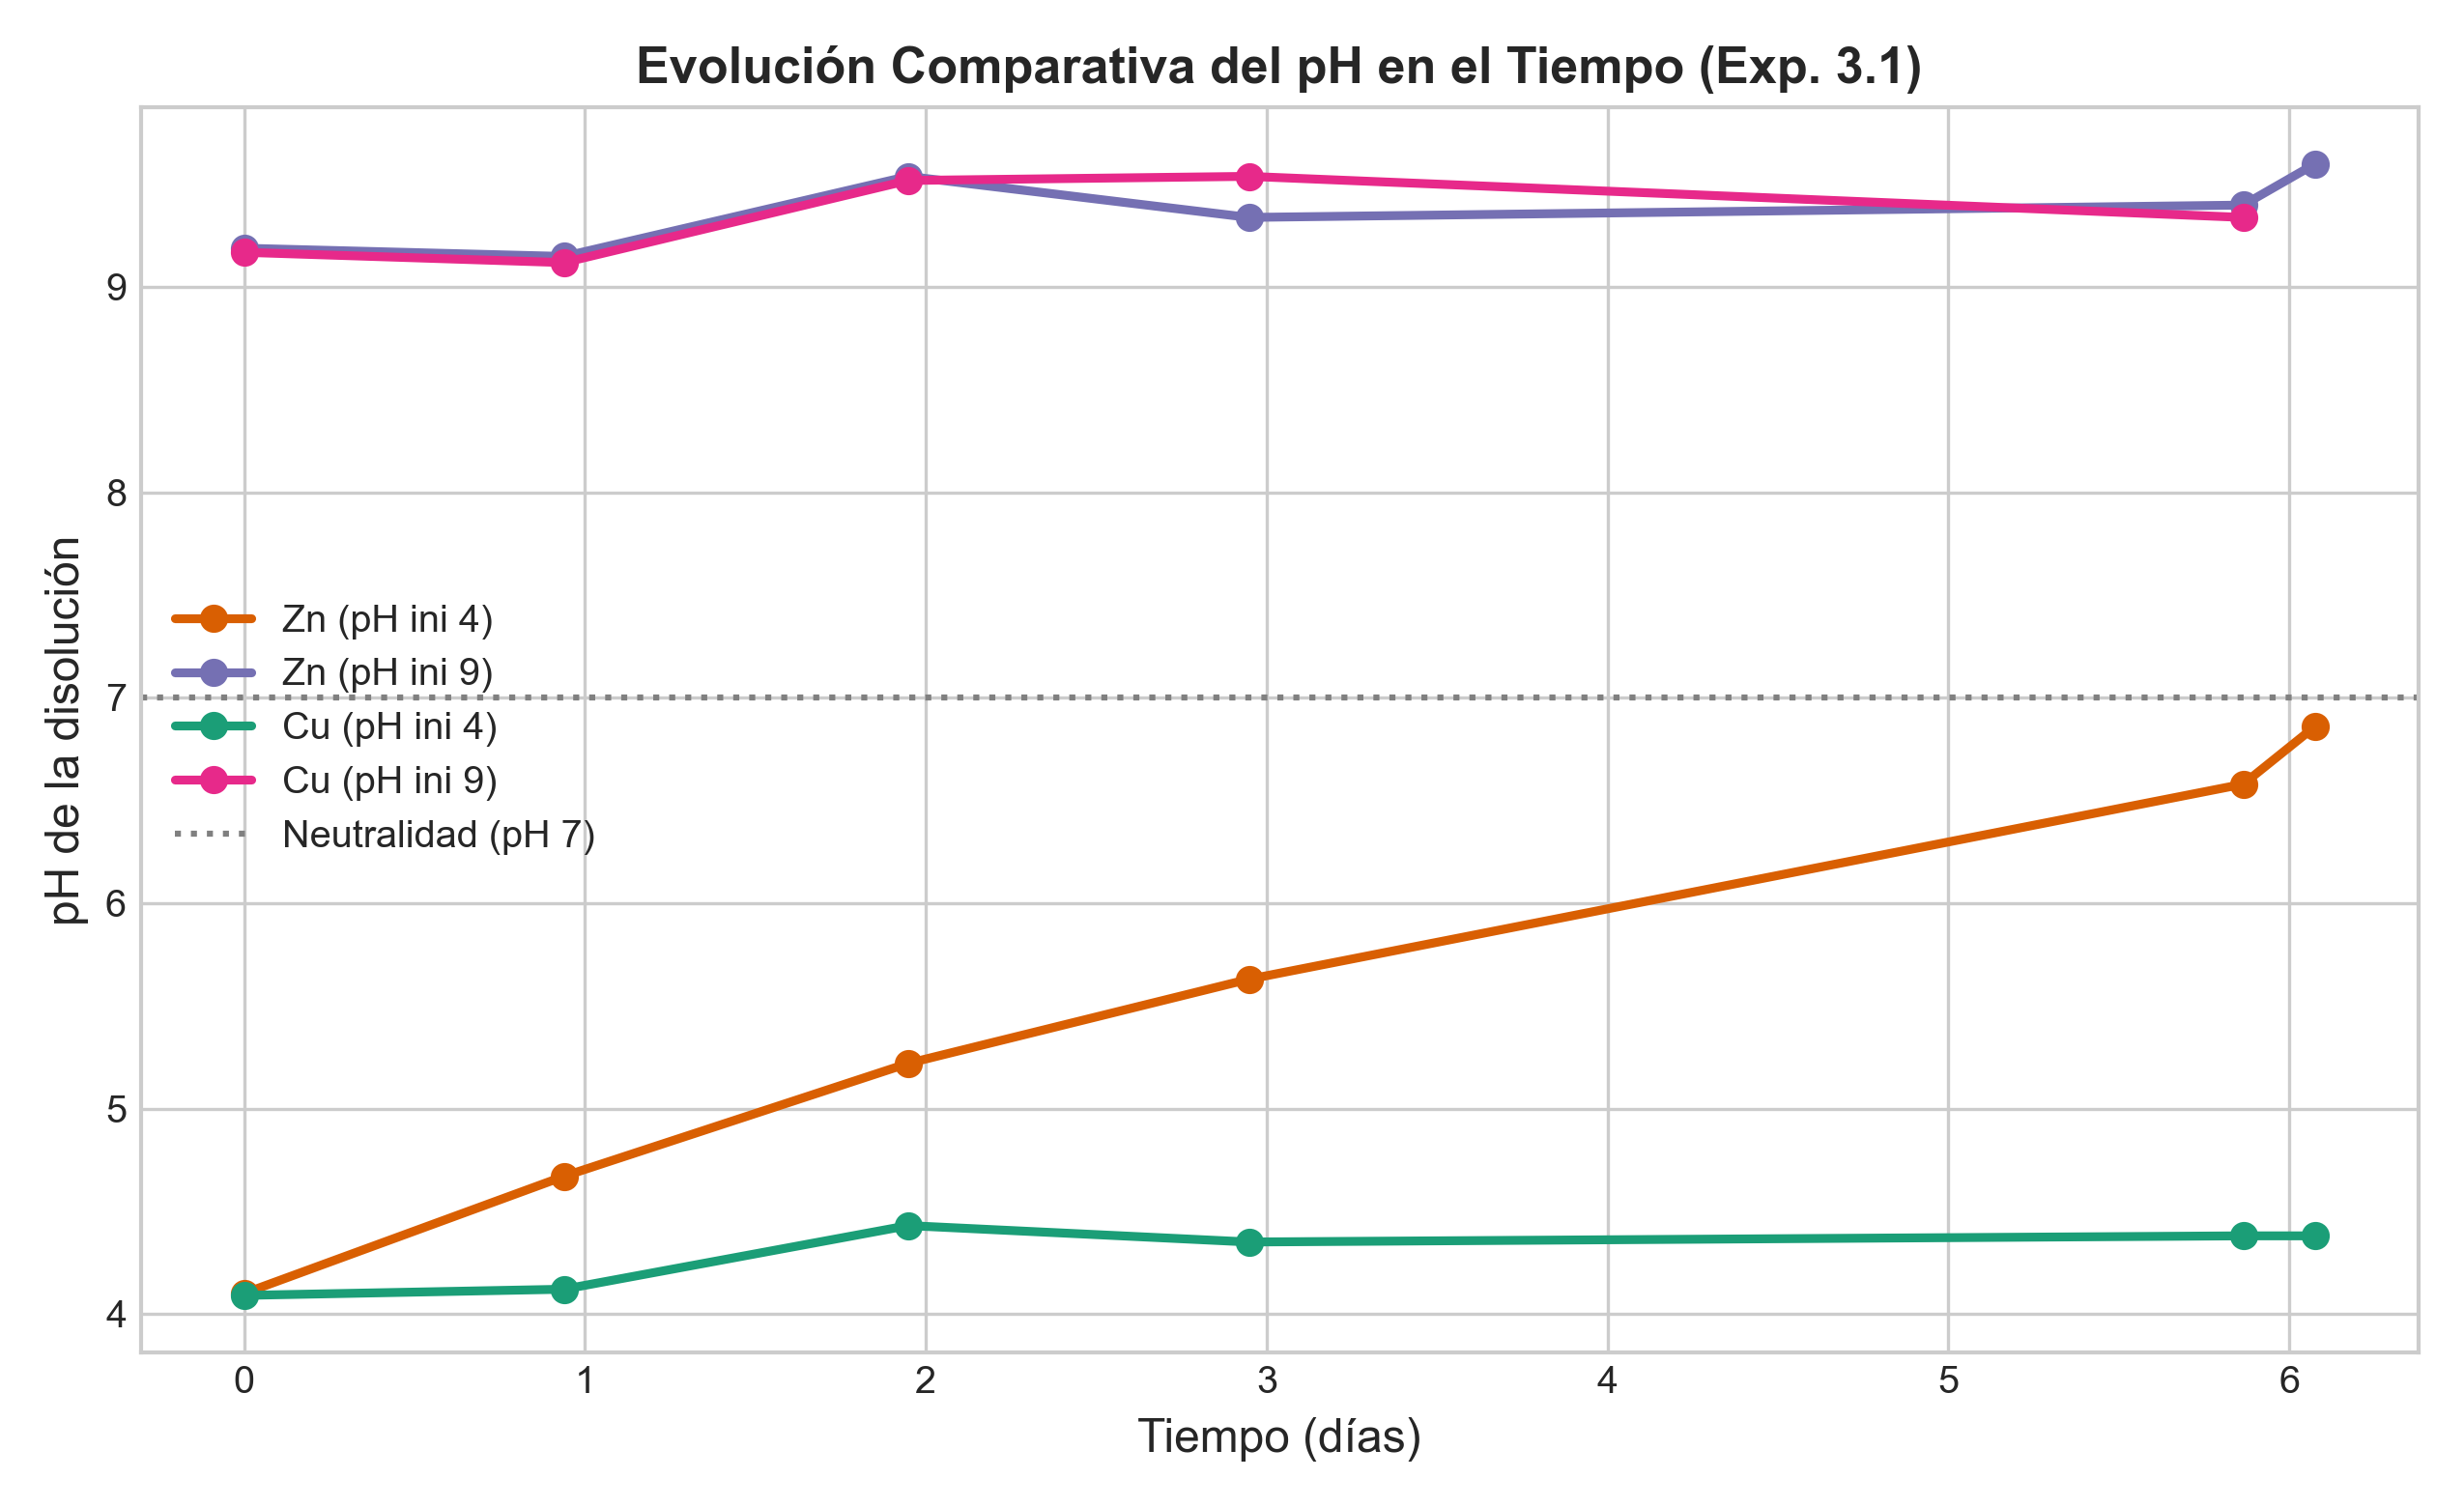
\includegraphics[width=0.82\textwidth]{resultados_practica_corrosion/exp_3_1_conjunto_pH.png}
    \caption{Evolución comparativa del pH en función del tiempo para todas las series del Experimento 3.1.}
    \label{fig:exp_3_1_pH}
\end{figure}

\begin{figure}[H]
    \centering
    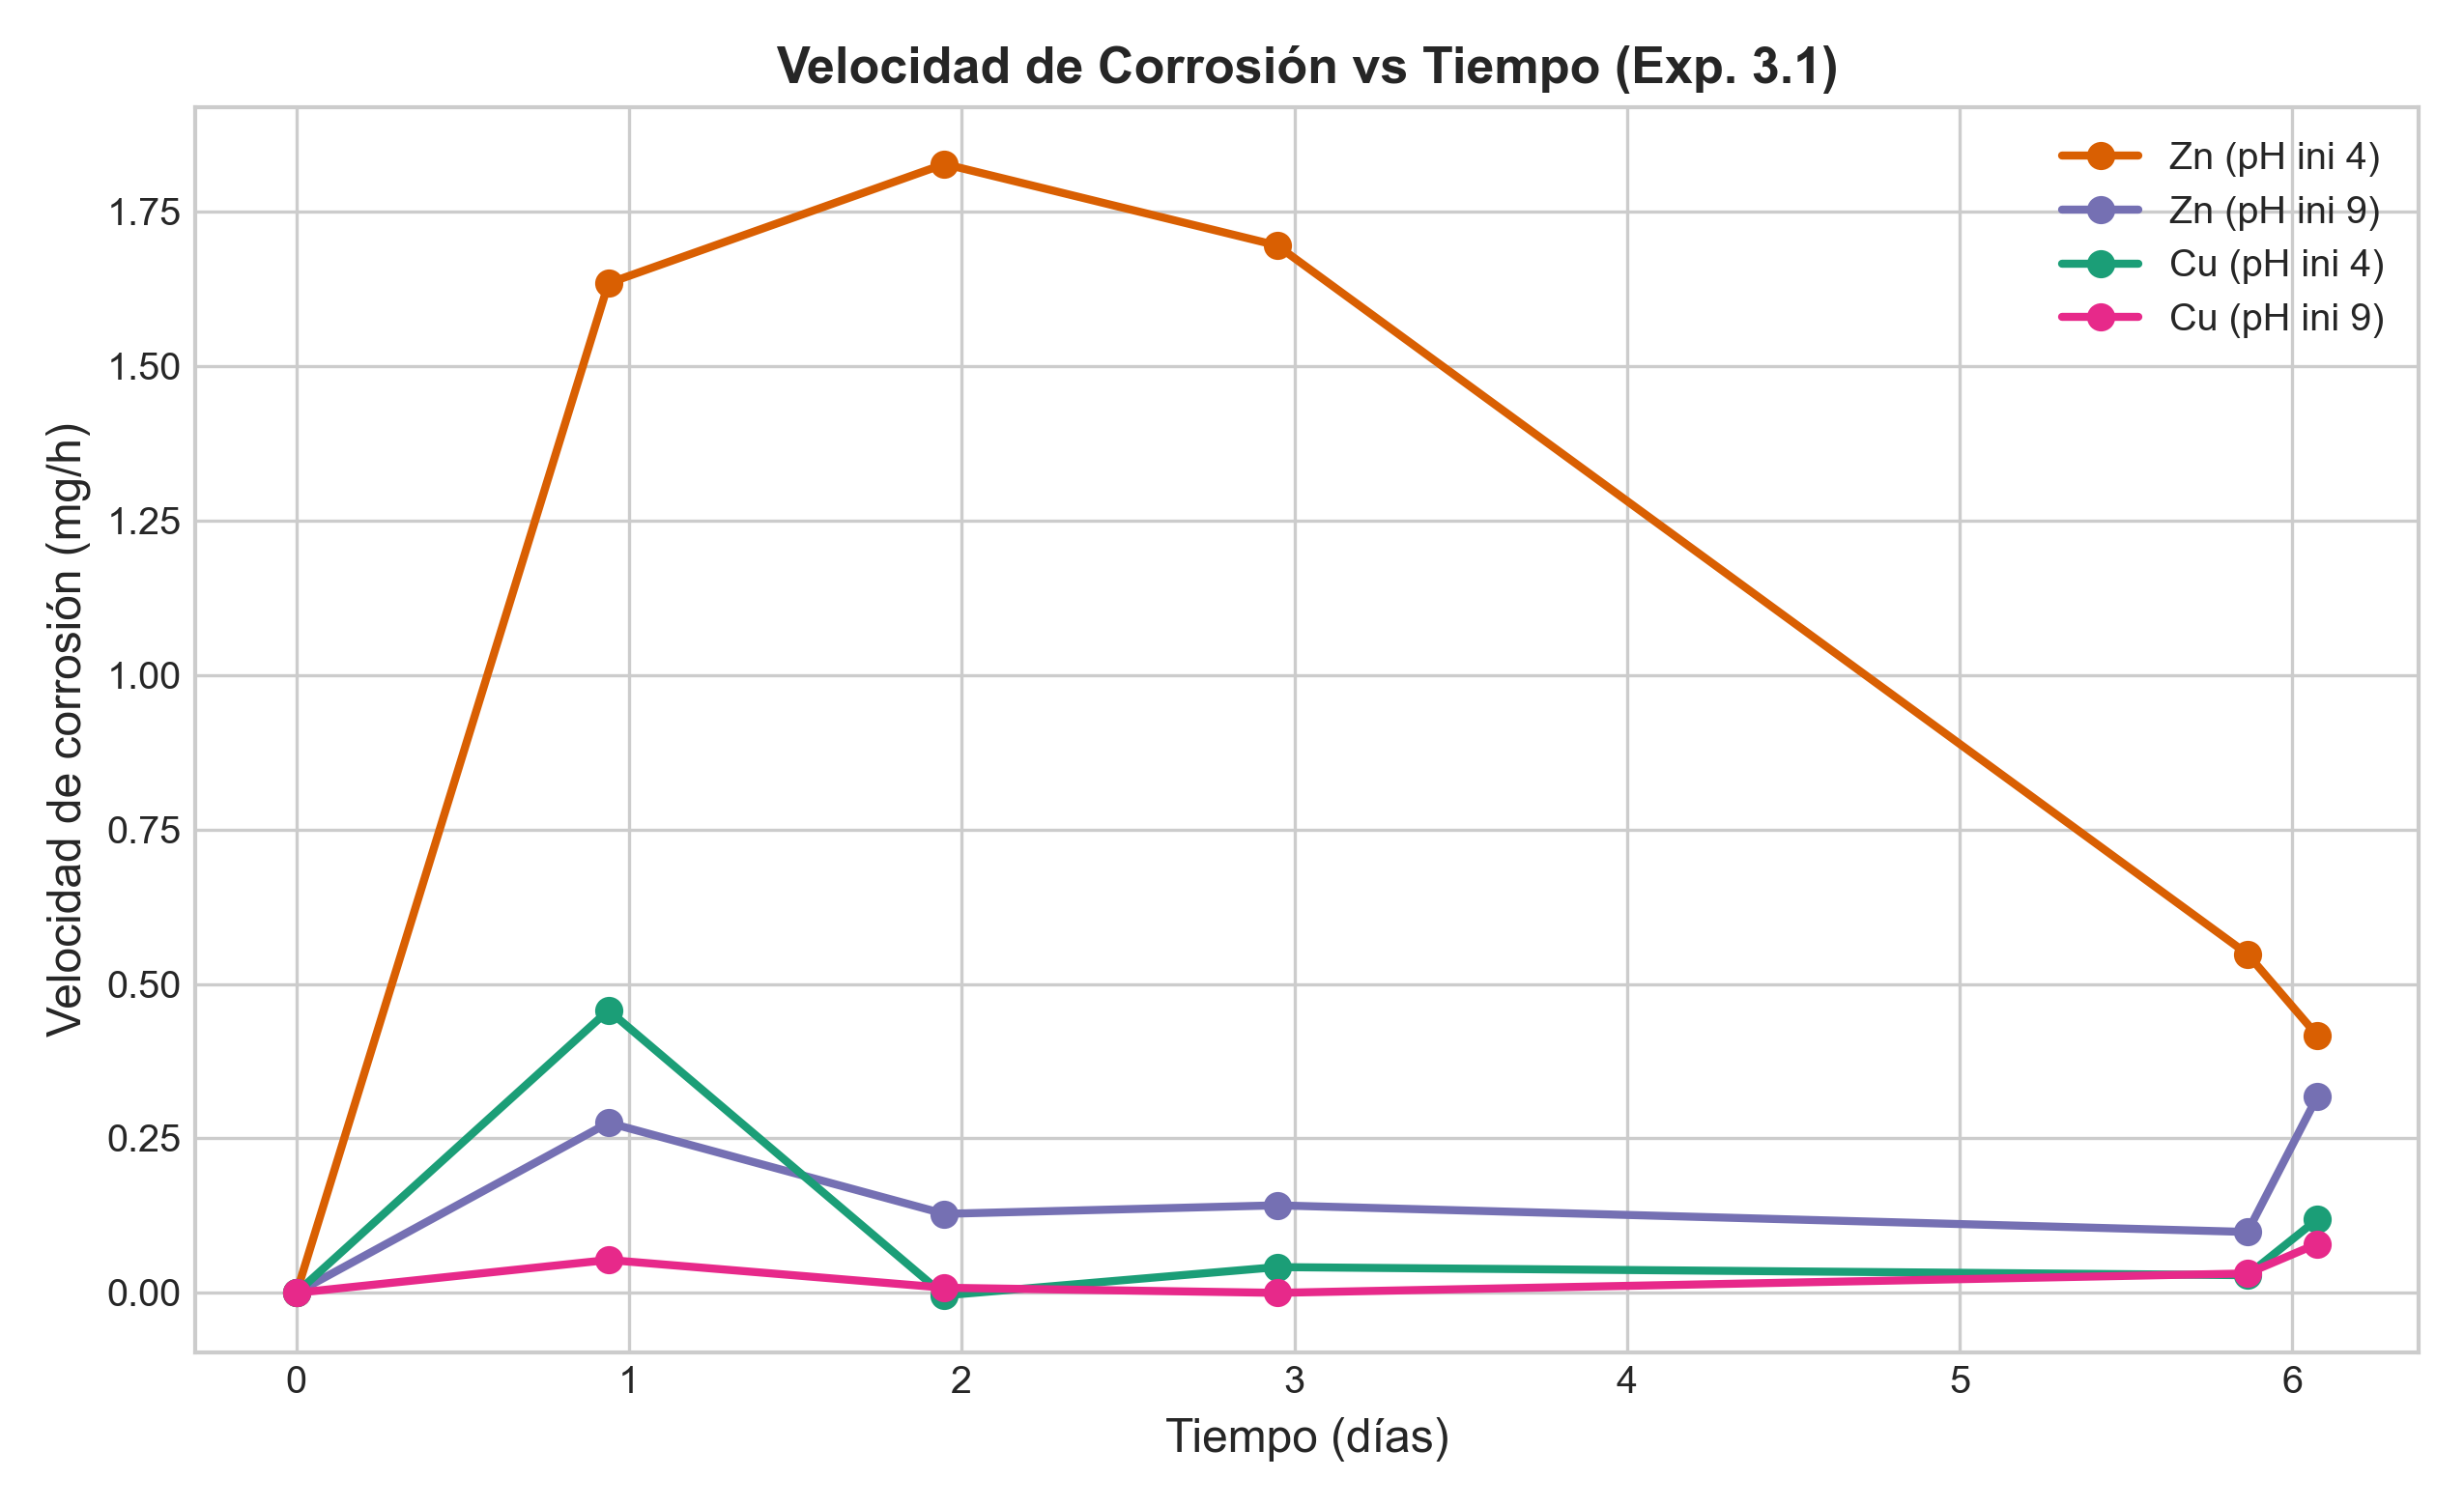
\includegraphics[width=0.82\textwidth]{resultados_practica_corrosion/exp_3_1_conjunto_velocidad.png}
    \caption{Velocidades de corrosión incrementales en función del tiempo para todas las series de Zn y Cu.}
    \label{fig:exp_3_1_vel}
\end{figure}

\begin{figure}[H]
    \centering
    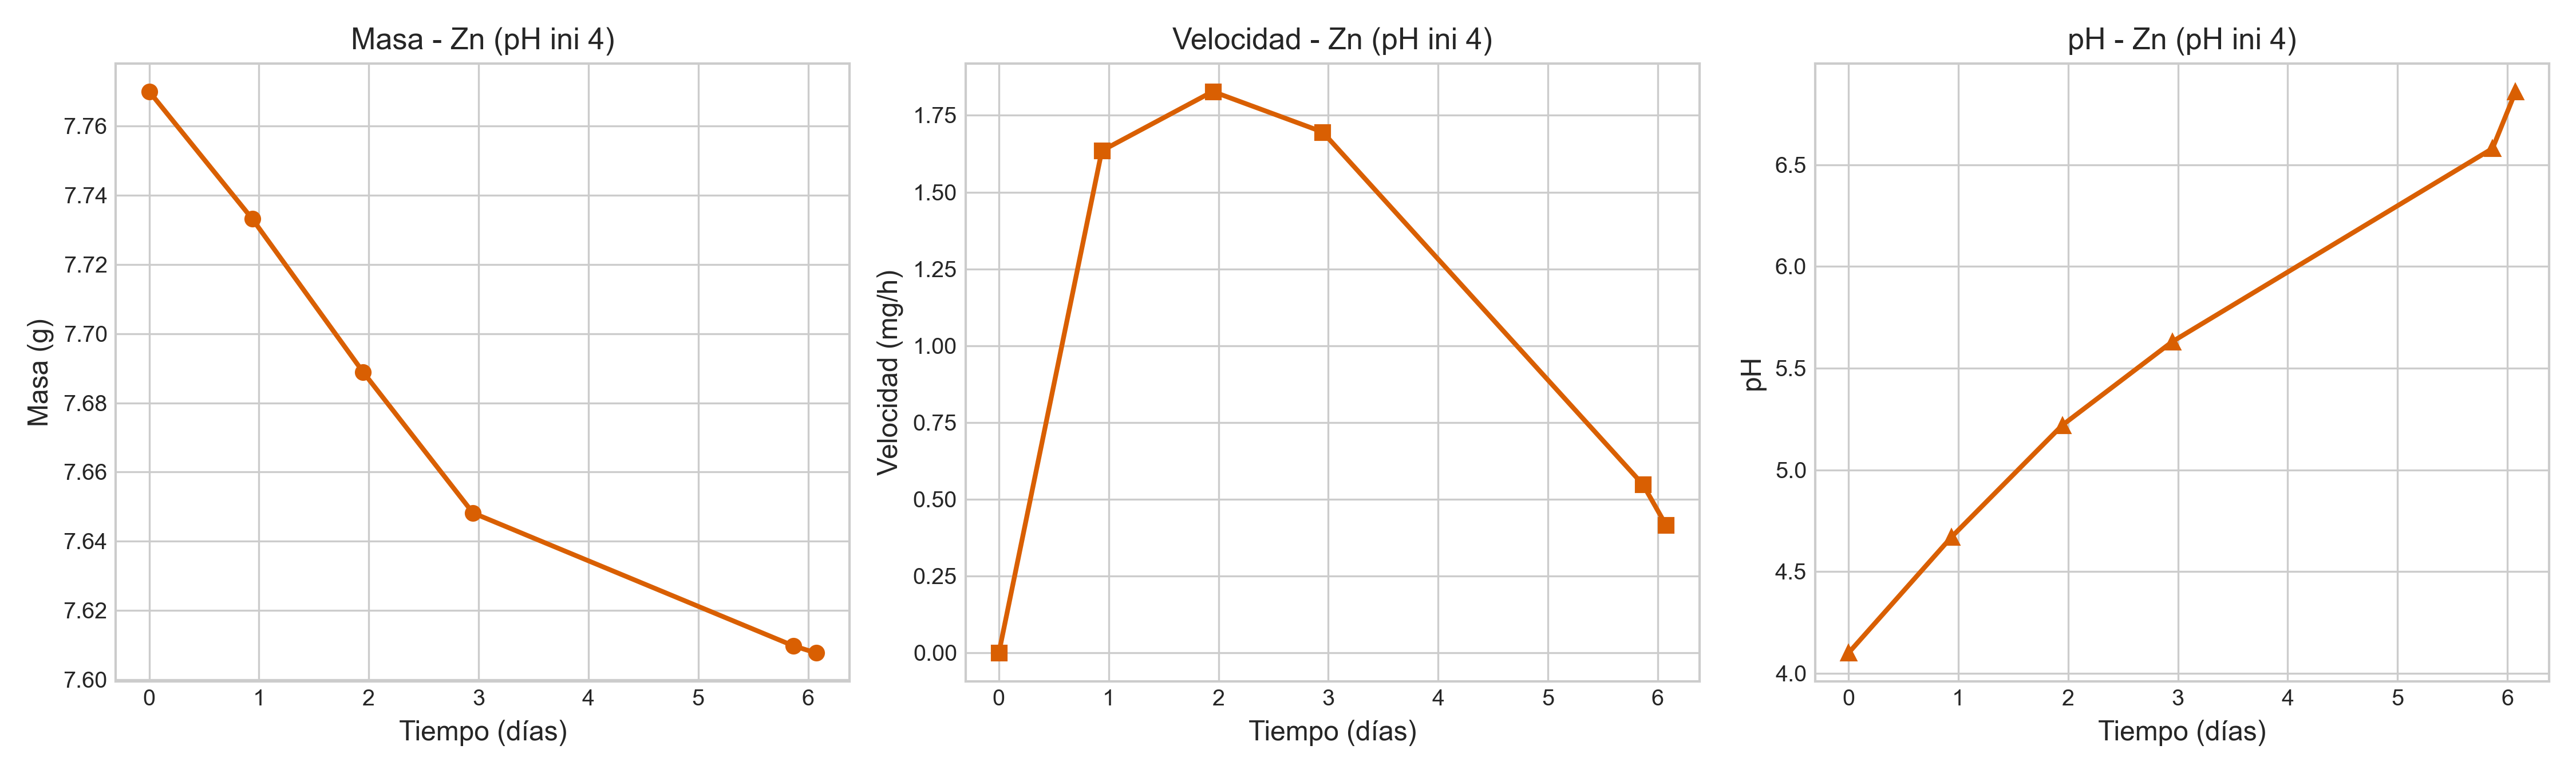
\includegraphics[width=0.95\textwidth]{resultados_practica_corrosion/exp_3_1_individual_Zn_pH4.png}
    \caption{Evolución individual de Masa, Velocidad y pH para Zinc a pH inicial 4.}
    \label{fig:exp_3_1_ind_zn4}
\end{figure}

\begin{figure}[H]
    \centering
    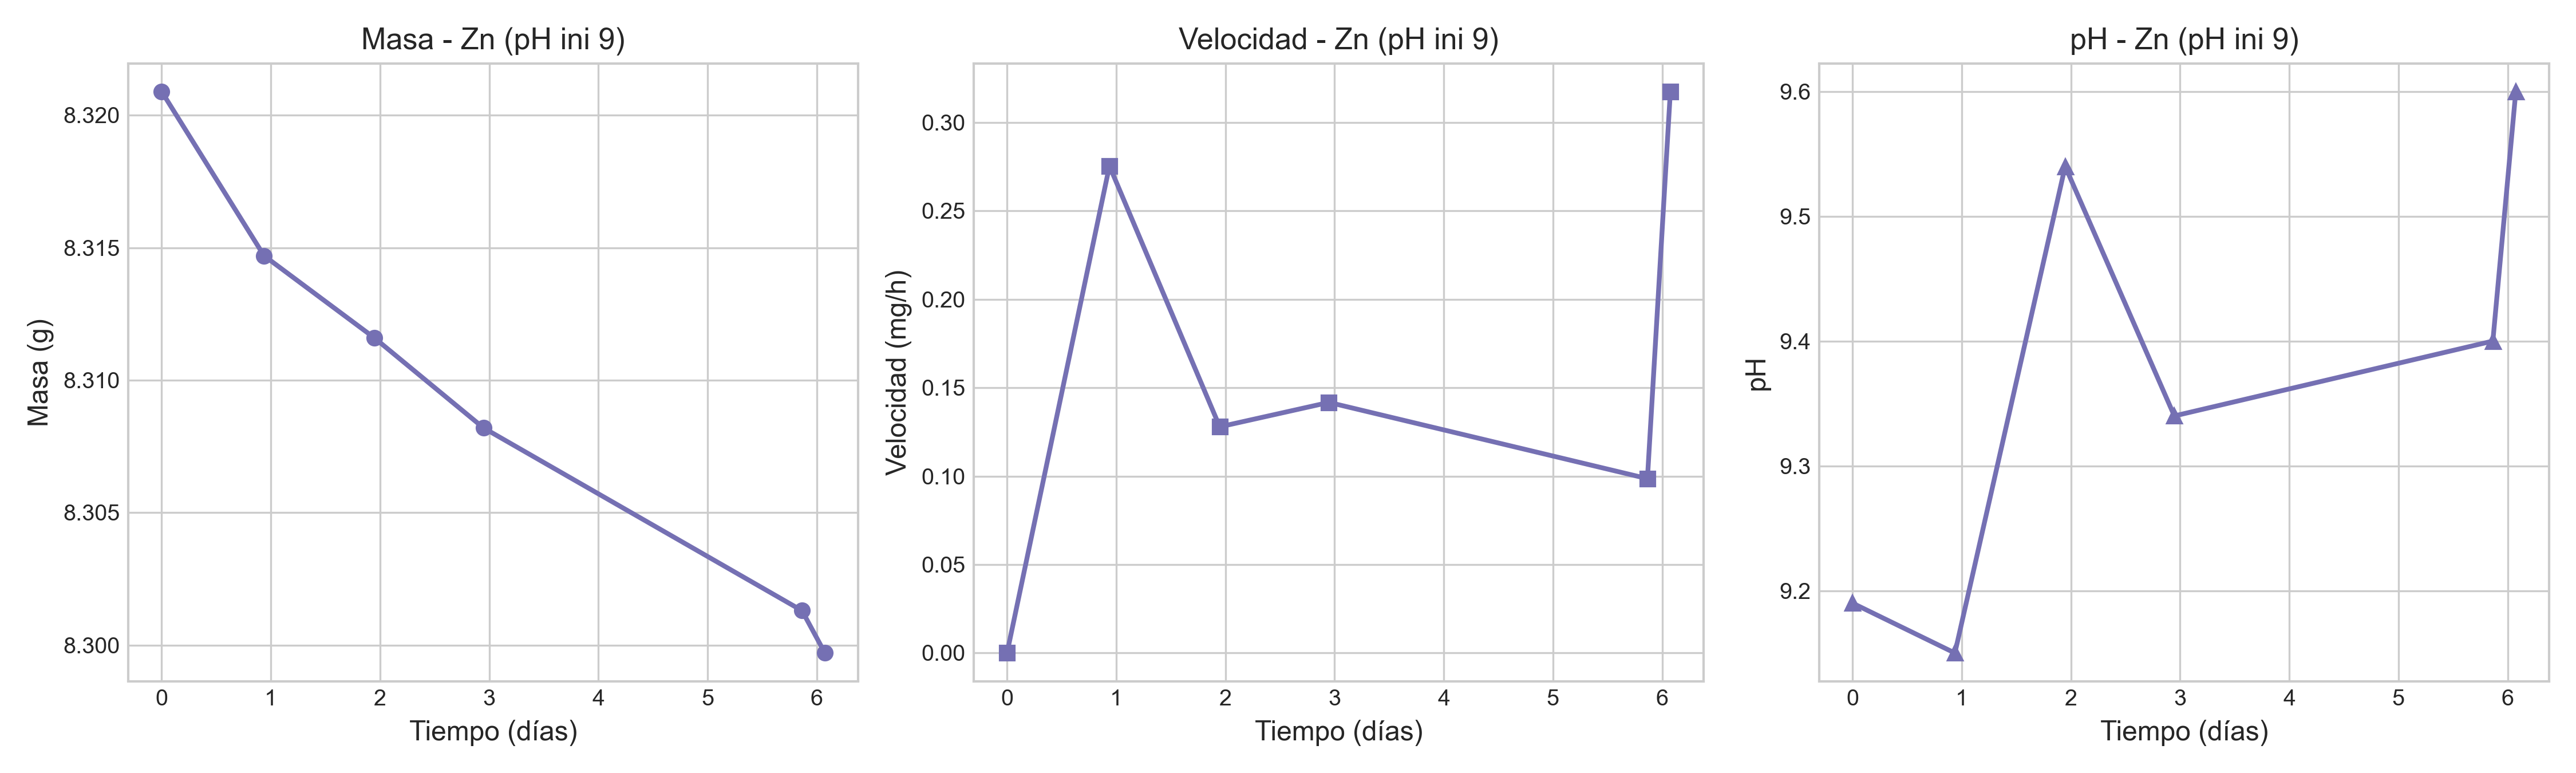
\includegraphics[width=0.95\textwidth]{resultados_practica_corrosion/exp_3_1_individual_Zn_pH9.png}
    \caption{Evolución individual de Masa, Velocidad y pH para Zinc a pH inicial 9.}
    \label{fig:exp_3_1_ind_zn9}
\end{figure}

\begin{figure}[H]
    \centering
    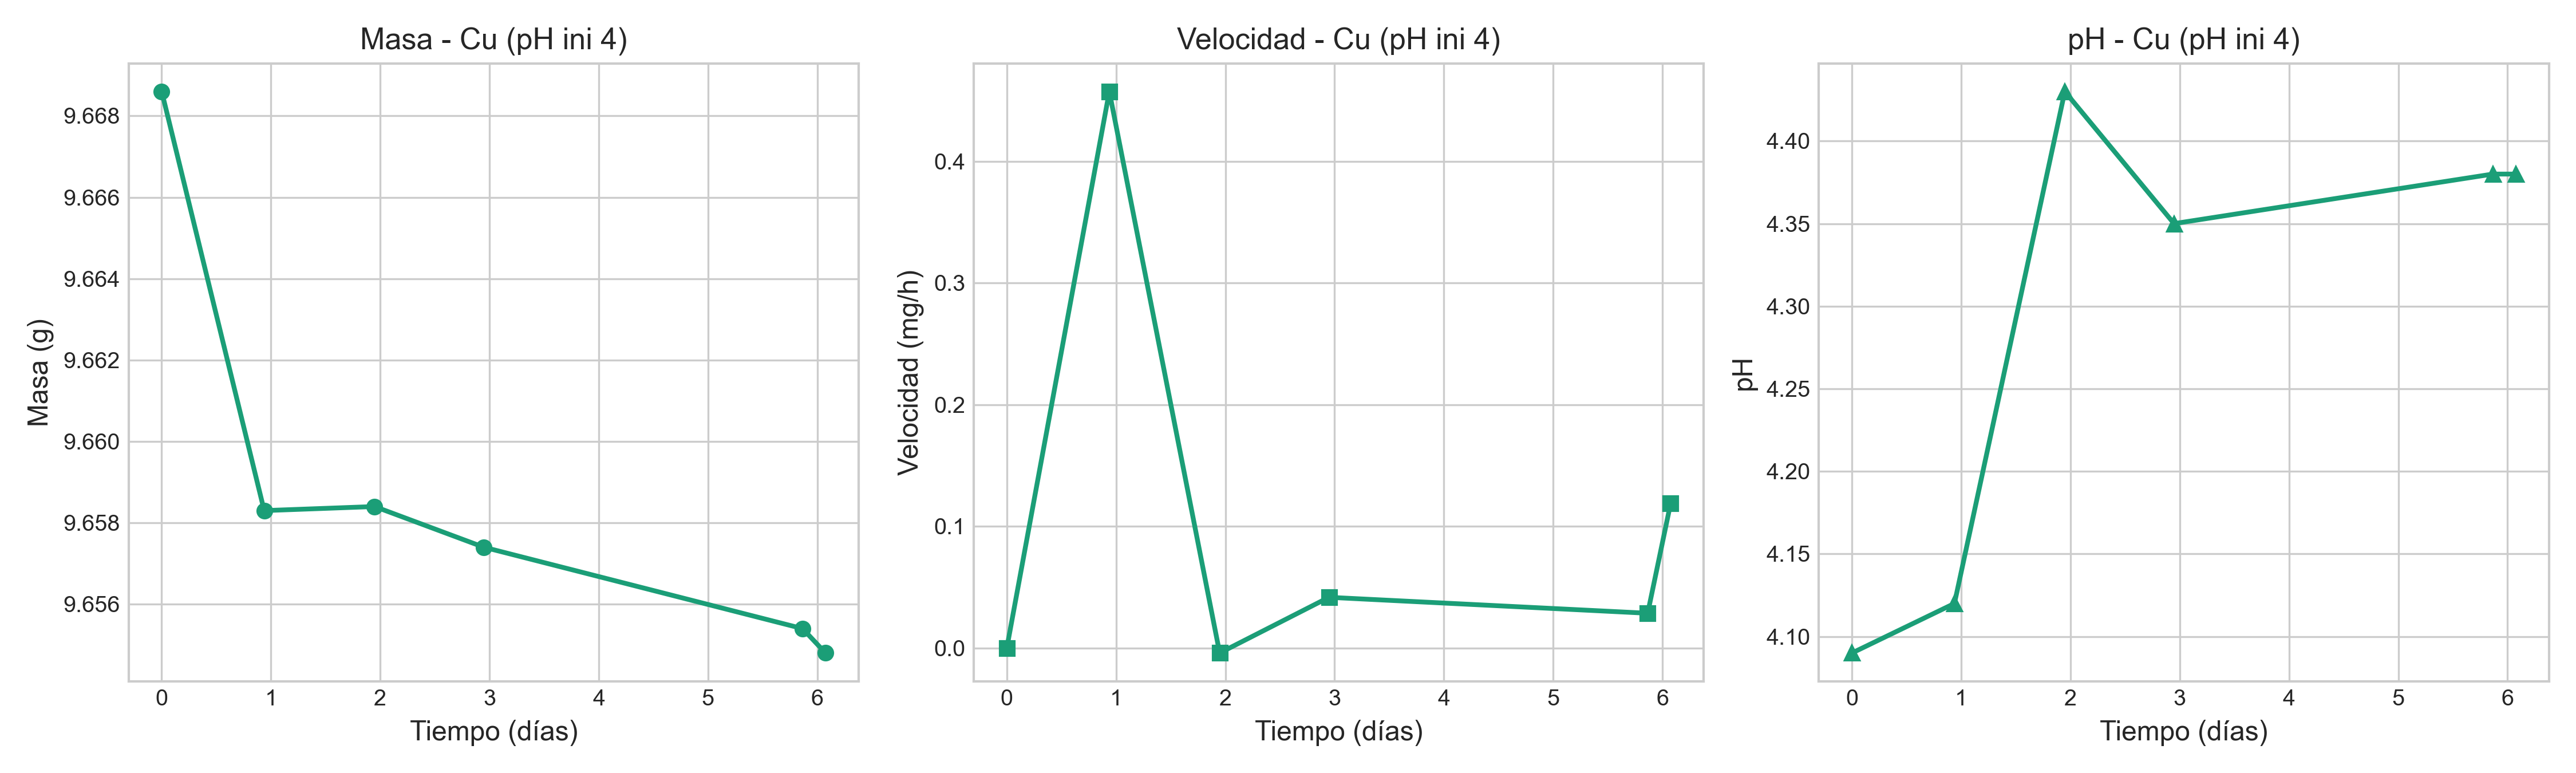
\includegraphics[width=0.95\textwidth]{resultados_practica_corrosion/exp_3_1_individual_Cu_pH4.png}
    \caption{Evolución individual de Masa, Velocidad y pH para Cobre a pH inicial 4.}
    \label{fig:exp_3_1_ind_cu4}
\end{figure}

\begin{figure}[H]
    \centering
    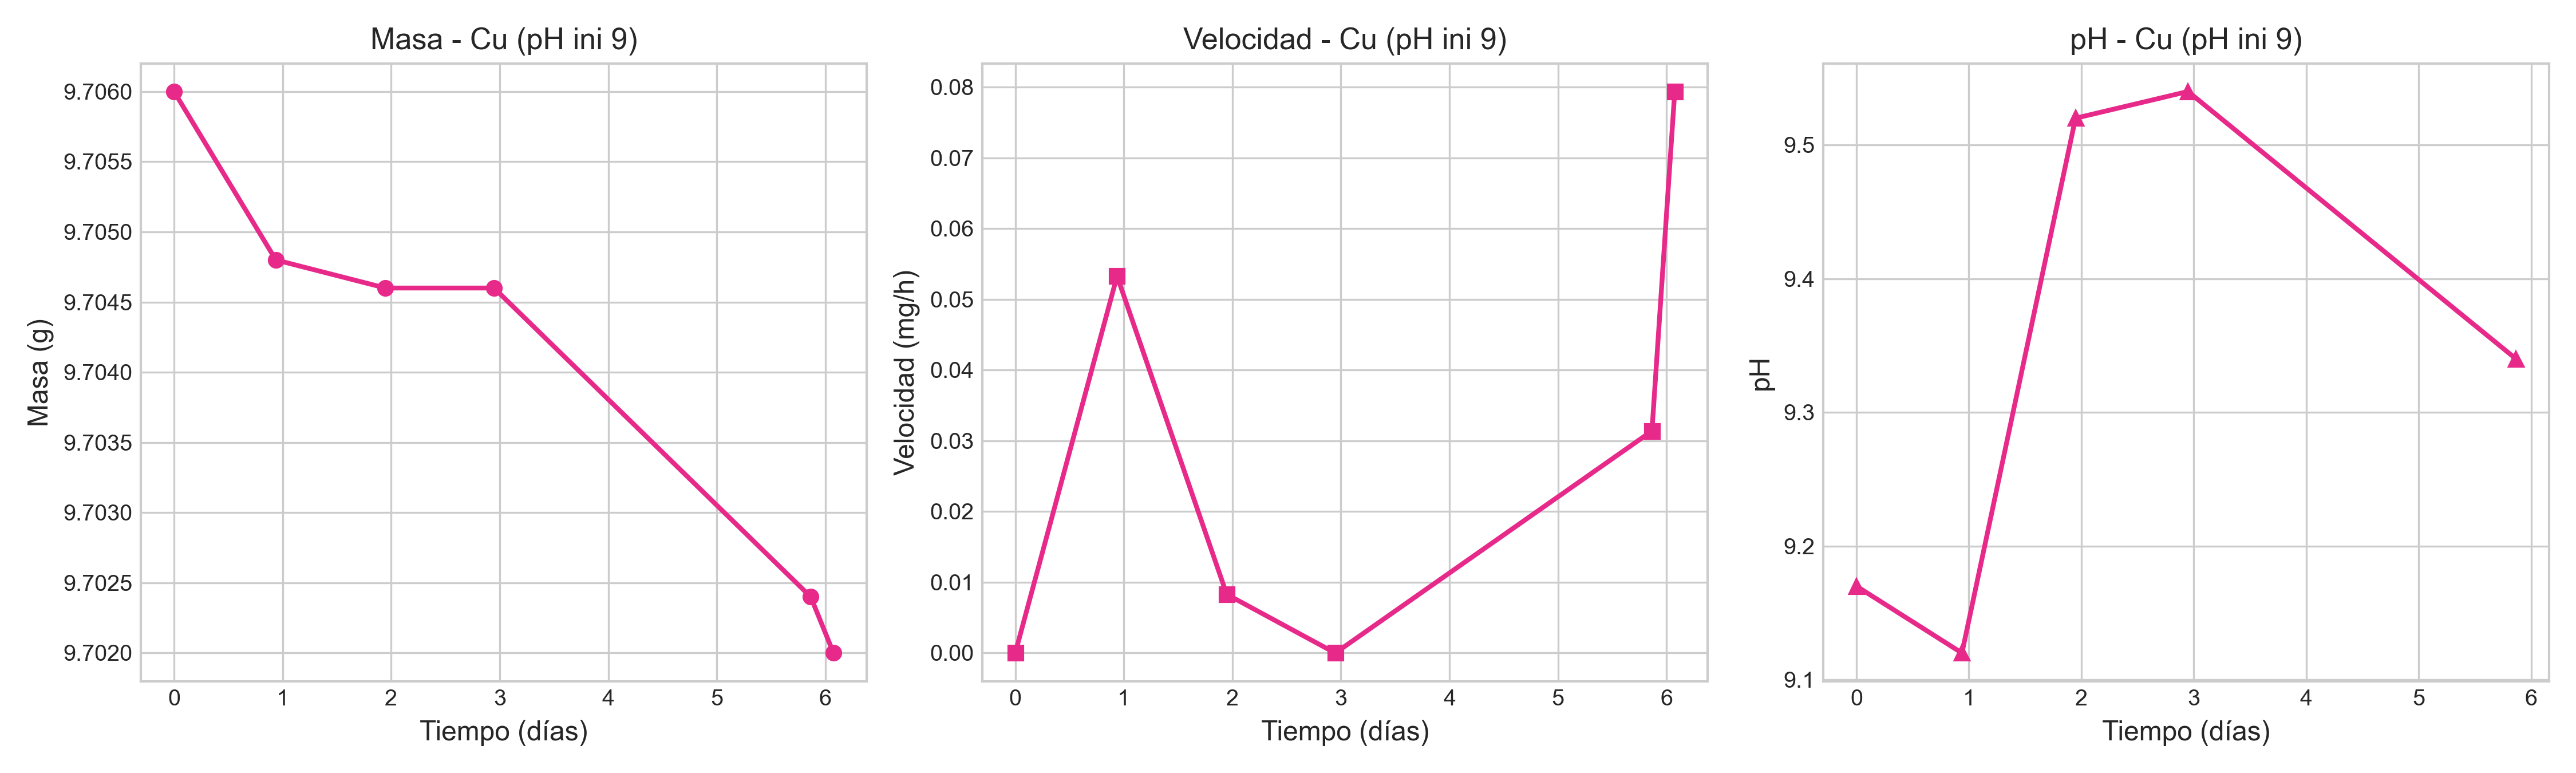
\includegraphics[width=0.95\textwidth]{resultados_practica_corrosion/exp_3_1_individual_Cu_pH9.png}
    \caption{Evolución individual de Masa, Velocidad y pH para Cobre a pH inicial 9.}
    \label{fig:exp_3_1_ind_cu9}
\end{figure}

% =============================================================================
\section{Experimento 3.2: Corrosión en Materiales Sometidos a Esfuerzos (Subgrupo A)}
% =============================================================================
\subsection{Fundamento y Mecanismo}
El mecanizado (taladrado o entallado) introduce deformación plástica localizada (\textit{strain hardening} / acritud) y elevadas tensiones mecánicas residuales de tracción.
\begin{itemize}
    \item La distorsión de la red cristalina eleva la energía libre de Gibbs superficial ($G$), convirtiendo el área tensionada en una zona termodinámicamente más activa (microánodo).
    \item Se forma un par galvánico microscópico local:
    \begin{align}
        \text{Ánodo local (zona deformada/taladro):} \quad & \text{Fe(s)} \longrightarrow \text{Fe}^{2+} + 2e^- \\
        \text{Cátodo local (matriz no deformada):} \quad & 2\text{H}^+ + 2e^- \longrightarrow \text{H}_2(\text{g})
    \end{align}
\end{itemize}
Como consecuencia, la probeta taladrada experimenta una velocidad de disolución notablemente superior en $\text{HCl}$ 2N frente a la probeta intacta.

\subsection{Resultados Experimentales y Gráficas}
\begin{table}[H]
\centering
\caption{Probeta de acero NO taladrada en $\text{HCl}$ 2N}
\label{tab:3_2_no_tal}
\begin{tabular}{cccccc}
\toprule
t (min) & t (h) & Masa (g) & Masa (\%) & Pérdida (mg) & Velocidad (mg/h) \\
\midrule
0.0000 & 0.0000 & 8.6398 & 100.00 & 0.0000 & 0.0000 \\
5.0000 & 0.0833 & 8.6396 & 99.9977 & 0.2000 & 2.4000 \\
15.0000 & 0.2500 & 8.6385 & 99.9850 & 1.3000 & 6.6000 \\
25.0000 & 0.4167 & 8.6371 & 99.9687 & 2.7000 & 8.4000 \\
35.0000 & 0.5833 & 8.6364 & 99.9606 & 3.4000 & 4.2000 \\
50.0000 & 0.8333 & 8.6356 & 99.9514 & 4.2000 & 3.2000 \\
65.0000 & 1.0833 & 8.6333 & 99.9248 & 6.5000 & 9.2000 \\
80.0000 & 1.3333 & 8.6329 & 99.9201 & 6.9000 & 1.6000 \\
107.00 & 1.7833 & 8.6297 & 99.8831 & 10.1000 & 7.1100 \\
132.00 & 2.2000 & 8.6293 & 99.8785 & 10.5000 & 0.9600 \\
145.00 & 2.4167 & 8.6278 & 99.8611 & 12.0000 & 6.9200 \\
165.00 & 2.7500 & 8.6279 & 99.8623 & 11.9000 & -0.3000 \\
185.00 & 3.0833 & 8.6270 & 99.8518 & 12.8000 & 2.7000 \\
205.00 & 3.4167 & 8.6252 & 99.8310 & 14.6000 & 5.4000 \\
225.00 & 3.7500 & 8.6245 & 99.8229 & 15.3000 & 2.1000 \\
245.00 & 4.0833 & 8.6230 & 99.8056 & 16.8000 & 4.5000 \\
\bottomrule
\end{tabular}
\end{table}

\begin{table}[H]
\centering
\caption{Probeta de acero TALADRADA en $\text{HCl}$ 2N}
\label{tab:3_2_tal}
\begin{tabular}{cccccc}
\toprule
t (min) & t (h) & Masa (g) & Masa (\%) & Pérdida (mg) & Velocidad (mg/h) \\
\midrule
0.0000 & 0.0000 & 8.3728 & 100.00 & 0.0000 & 0.0000 \\
5.0000 & 0.0833 & 8.3719 & 99.9893 & 0.9000 & 10.8000 \\
15.0000 & 0.2500 & 8.3702 & 99.9689 & 2.6000 & 10.2000 \\
25.0000 & 0.4167 & 8.3689 & 99.9534 & 3.9000 & 7.8000 \\
35.0000 & 0.5833 & 8.3675 & 99.9367 & 5.3000 & 8.4000 \\
50.0000 & 0.8333 & 8.3659 & 99.9176 & 6.9000 & 6.4000 \\
65.0000 & 1.0833 & 8.3641 & 99.8961 & 8.7000 & 7.2000 \\
80.0000 & 1.3333 & 8.3625 & 99.8770 & 10.3000 & 6.4000 \\
107.00 & 1.7833 & 8.3589 & 99.8340 & 13.9000 & 8.0000 \\
132.00 & 2.2000 & 8.3568 & 99.8089 & 16.0000 & 5.0400 \\
145.00 & 2.4167 & 8.3565 & 99.8053 & 16.3000 & 1.3800 \\
165.00 & 2.7500 & 8.3542 & 99.7779 & 18.6000 & 6.9000 \\
185.00 & 3.0833 & 8.3530 & 99.7635 & 19.8000 & 3.6000 \\
205.00 & 3.4167 & 8.3517 & 99.7480 & 21.1000 & 3.9000 \\
225.00 & 3.7500 & 8.3509 & 99.7384 & 21.9000 & 2.4000 \\
245.00 & 4.0833 & 8.3508 & 99.7372 & 22.0000 & 0.3000 \\
\bottomrule
\end{tabular}
\end{table}


\begin{figure}[H]
    \centering
    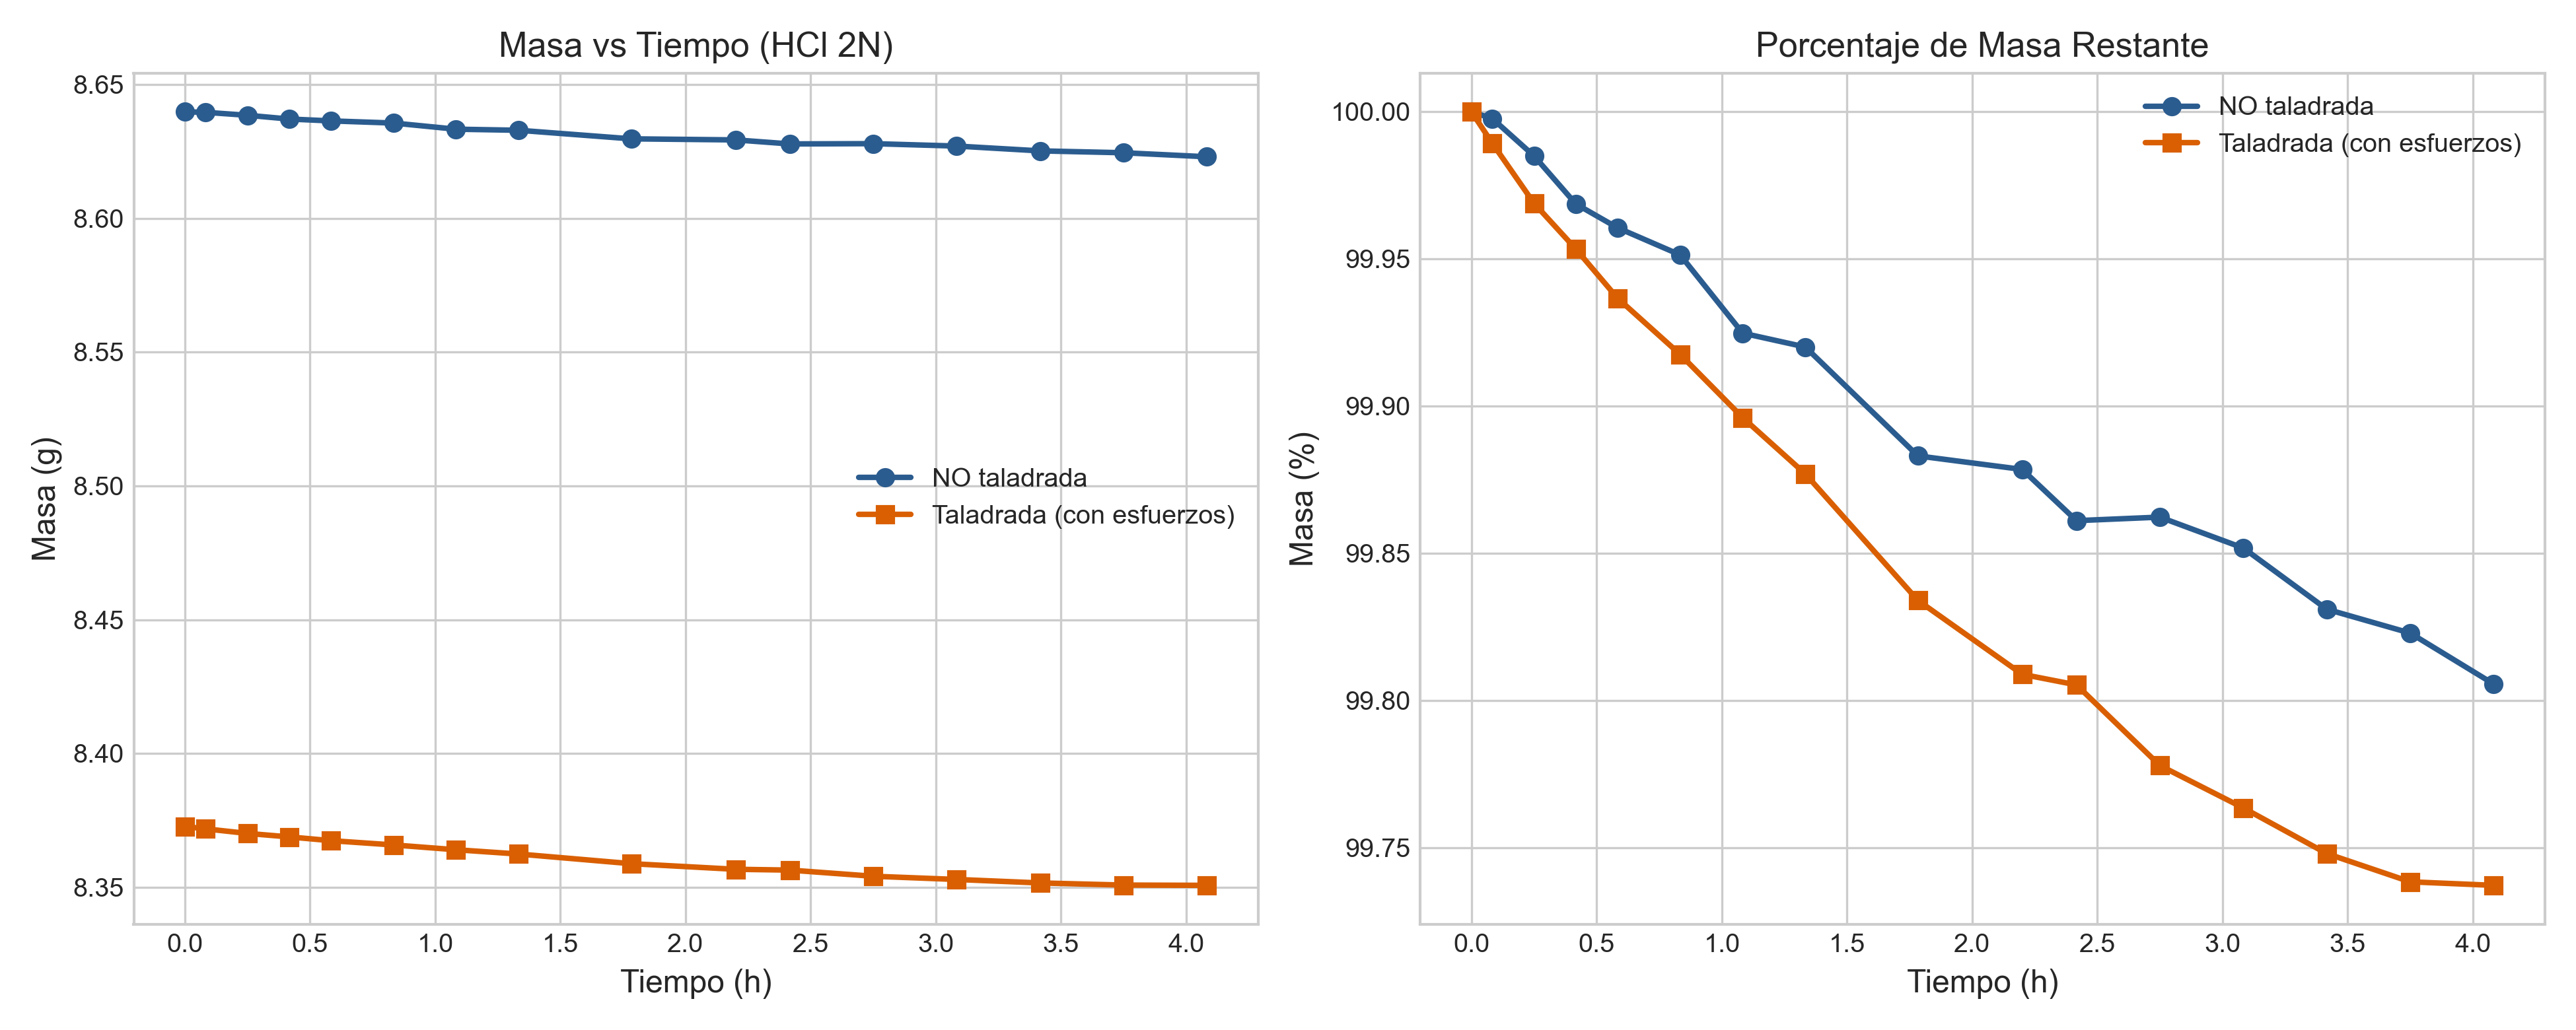
\includegraphics[width=0.92\textwidth]{resultados_practica_corrosion/exp_3_2_masa_y_pct.png}
    \caption{Comparativa de masa absoluta (g) y porcentaje restante (\%) en probetas con y sin concentración de esfuerzos.}
    \label{fig:exp_3_2_masa}
\end{figure}

\begin{figure}[H]
    \centering
    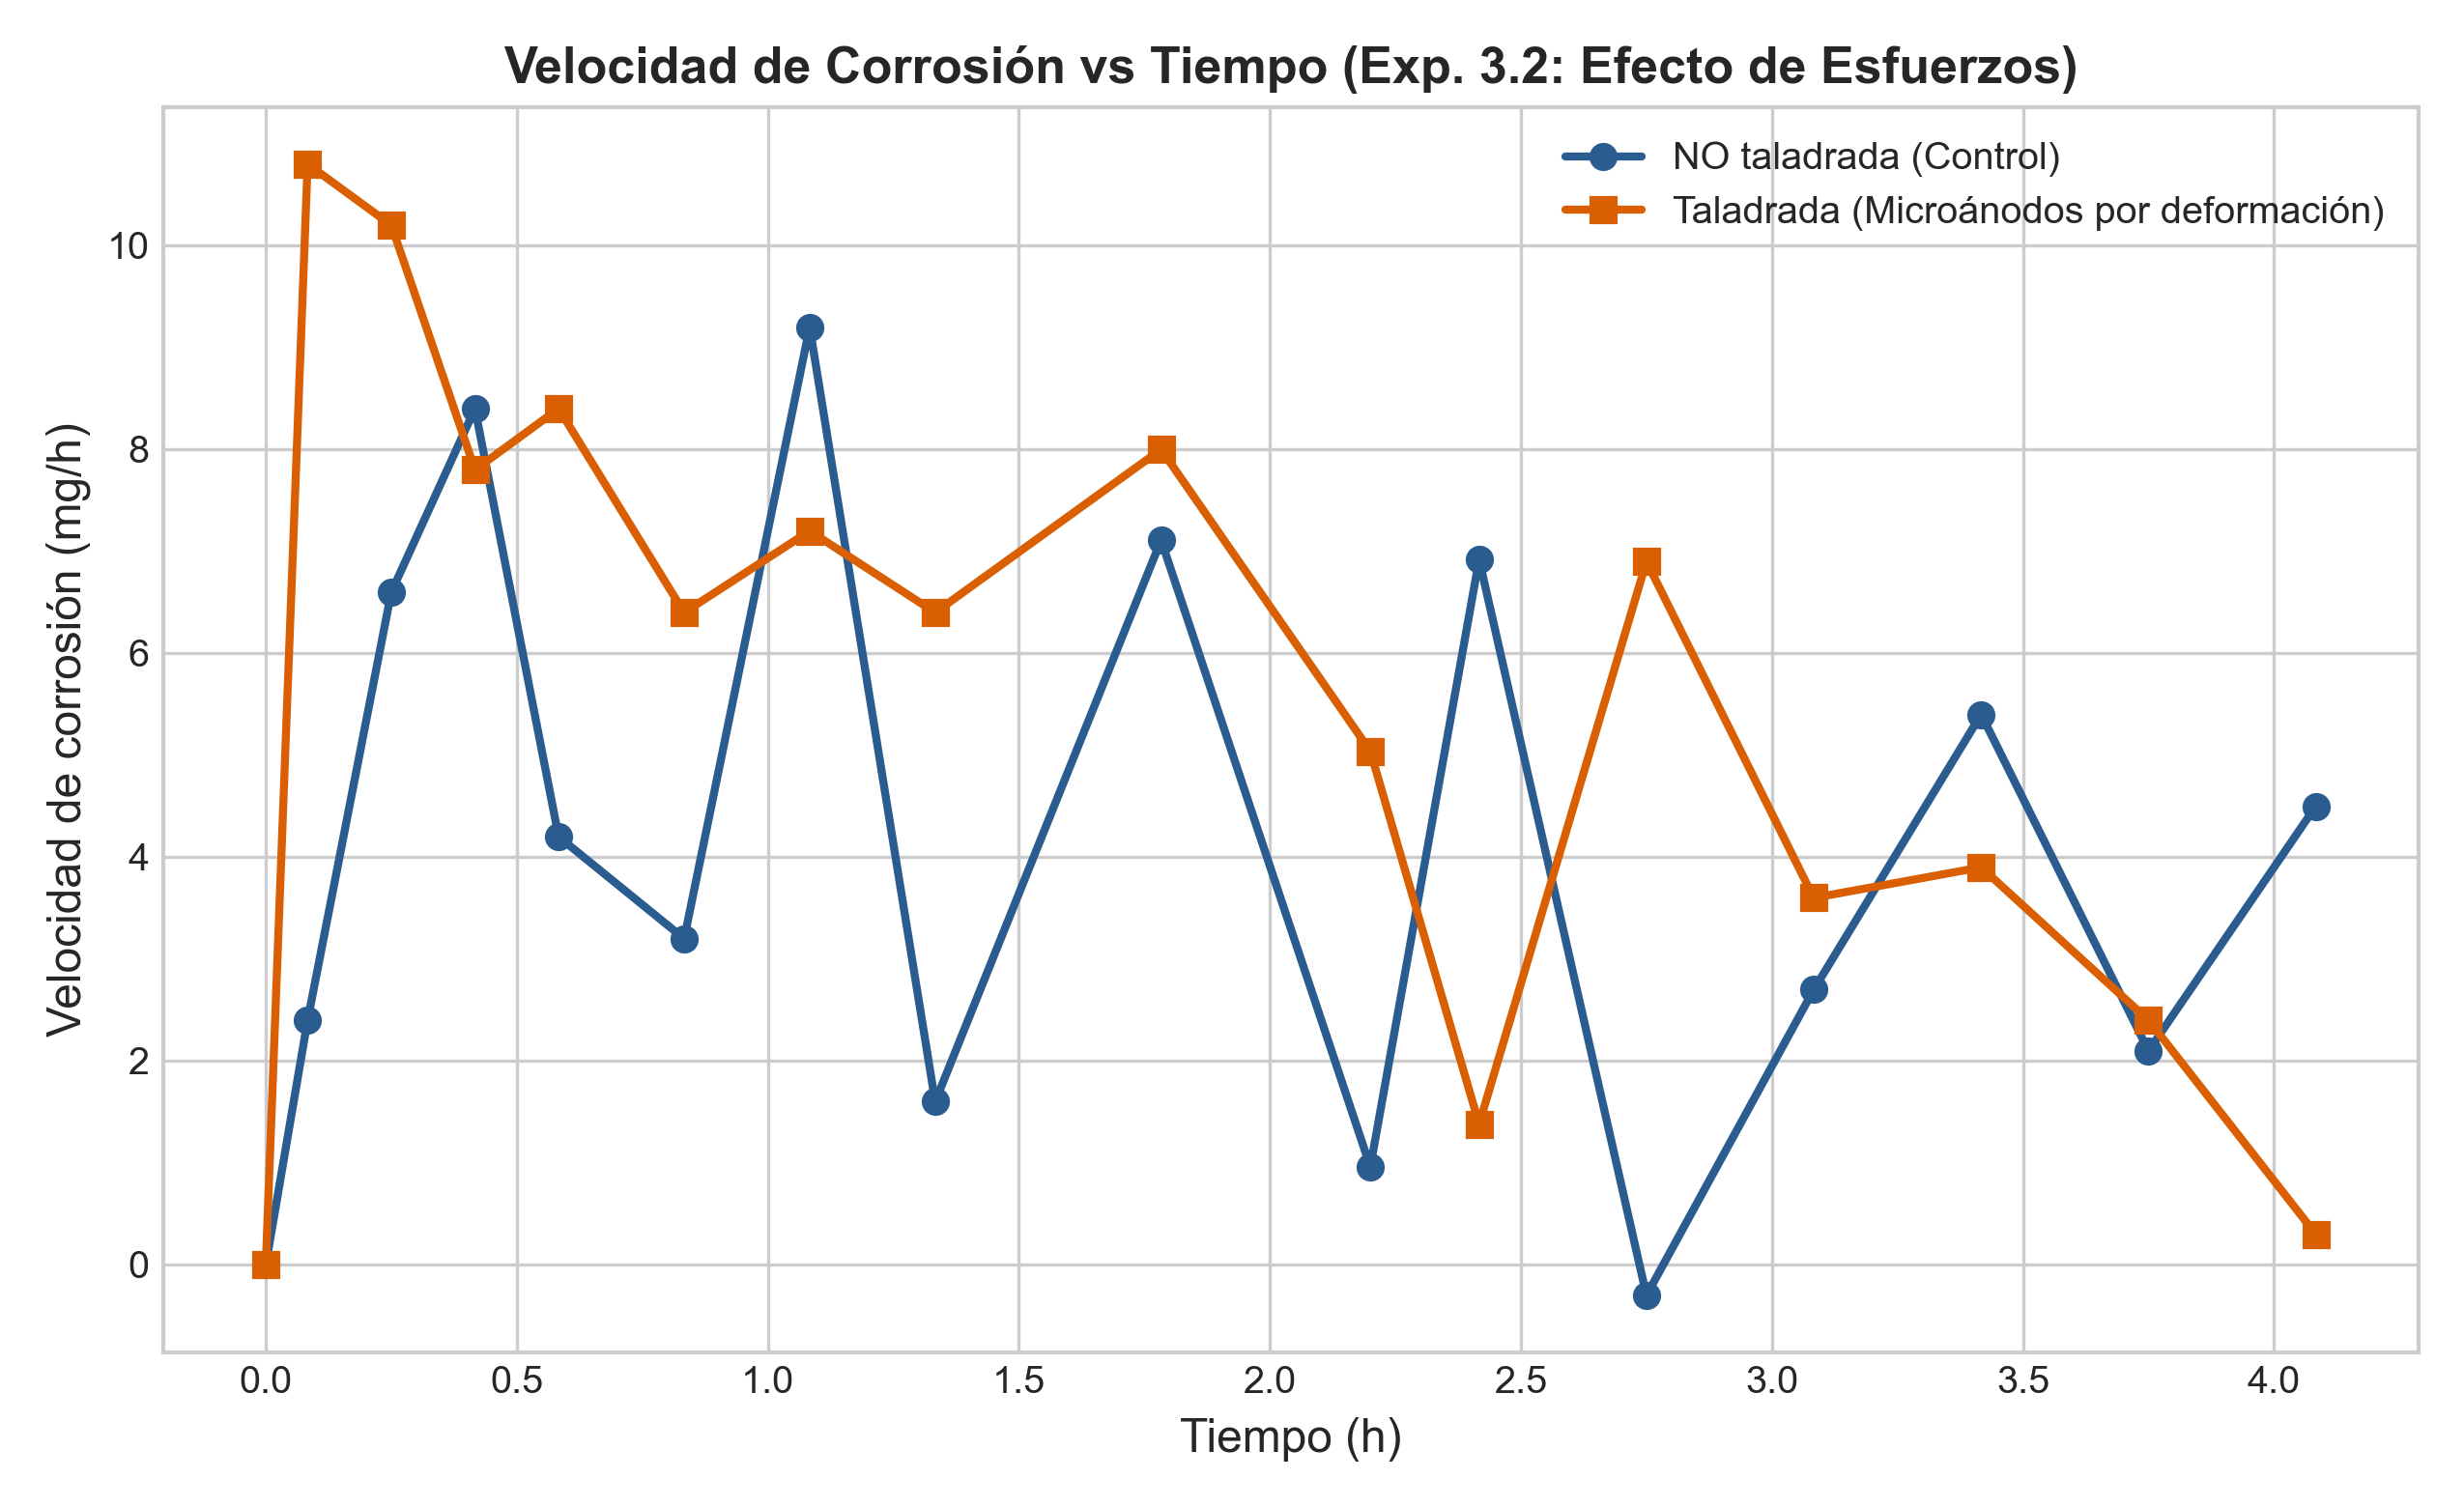
\includegraphics[width=0.82\textwidth]{resultados_practica_corrosion/exp_3_2_velocidad.png}
    \caption{Velocidad de corrosión incremental vs tiempo en probeta no taladrada vs taladrada.}
    \label{fig:exp_3_2_vel}
\end{figure}

% =============================================================================
\section{Experimento 3.3: Influencia del Oxígeno en la Corrosión del Acero (Subgrupo B)}
% =============================================================================
\subsection{Fundamento y Reacciones}
En soluciones salinas neutras ($\text{NaCl}$ 2M), el oxígeno disuelto actúa como el reactivo despolarizante fundamental de la reacción catódica:
\begin{align}
    \text{Oxidación anódica:} \quad & \text{Fe(s)} \longrightarrow \text{Fe}^{2+}(\text{aq}) + 2e^- \quad (E^0 = -0.44\text{ V}) \\
    \text{Reducción catódica (Aireada):} \quad & \text{O}_2 + 2\text{H}_2\text{O} + 4e^- \longrightarrow 4\text{OH}^- \quad (E^0 = +0.401\text{ V}) \\
    \text{Reacción global:} \quad & 2\text{Fe} + \text{O}_2 + 2\text{H}_2\text{O} \longrightarrow 2\text{Fe(OH)}_2(\text{s}) \xrightarrow{\text{O}_2} \text{Fe}_2\text{O}_3\cdot n\text{H}_2\text{O}
\end{align}
En la disolución \textbf{desaireada por ebullición}, la ausencia de $\text{O}_2$ disuelto inhibe el proceso catódico, ya que a pH neutro el sobrepotencial de reducción de protones ($2\text{H}_2\text{O} + 2e^- \rightarrow \text{H}_2 + 2\text{OH}^-$) es excesivamente alto para permitir una cinética apreciable. Por tanto, la corrosión en medio desaireado se detiene prácticamente por control catódico difusional.

\subsection{Resultados Experimentales y Gráficas}
\begin{table}[H]
\centering
\caption{Muestra 1 -- Disolución desaireada ($	ext{NaCl}$ 2M)}
\label{tab:3_3_des1}
\begin{tabular}{cccccc}
\toprule
t (min) & t (h) & Masa (g) & Masa (\%) & Pérdida (mg) & Velocidad (mg/h) \\
\midrule
0.0000 & 0.0000 & 8.1719 & 100.00 & 0.0000 & 0.0000 \\
15.0000 & 0.2500 & 8.1721 & 100.00 & -0.2000 & -0.8000 \\
30.0000 & 0.5000 & 8.1718 & 99.9988 & 0.1000 & 1.2000 \\
45.0000 & 0.7500 & 8.1715 & 99.9951 & 0.4000 & 1.2000 \\
60.0000 & 1.0000 & 8.1715 & 99.9951 & 0.4000 & -0.0000 \\
75.0000 & 1.2500 & 8.1713 & 99.9927 & 0.6000 & 0.8000 \\
129.00 & 2.1500 & 8.1717 & 99.9976 & 0.2000 & -0.4400 \\
149.00 & 2.4833 & 8.1710 & 99.9890 & 0.9000 & 2.1000 \\
169.00 & 2.8167 & 8.1713 & 99.9927 & 0.6000 & -0.9000 \\
192.00 & 3.2000 & 8.1707 & 99.9853 & 1.2000 & 1.5700 \\
209.00 & 3.4833 & 8.1663 & 99.9315 & 5.6000 & 15.5300 \\
227.00 & 3.7833 & 8.1673 & 99.9437 & 4.6000 & -3.3300 \\
244.00 & 4.0667 & 8.1663 & 99.9315 & 5.6000 & 3.5300 \\
255.00 & 4.2500 & 8.1661 & 99.9290 & 5.8000 & 1.0900 \\
\bottomrule
\end{tabular}
\end{table}

\begin{table}[H]
\centering
\caption{Muestra 2 -- Disolución desaireada ($	ext{NaCl}$ 2M)}
\label{tab:3_3_des2}
\begin{tabular}{cccccc}
\toprule
t (min) & t (h) & Masa (g) & Masa (\%) & Pérdida (mg) & Velocidad (mg/h) \\
\midrule
0.0000 & 0.0000 & 8.4685 & 100.00 & 0.0000 & 0.0000 \\
15.0000 & 0.2500 & 8.4688 & 100.00 & -0.3000 & -1.2000 \\
30.0000 & 0.5000 & 8.4679 & 99.9929 & 0.6000 & 3.6000 \\
45.0000 & 0.7500 & 8.4675 & 99.9882 & 1.0000 & 1.6000 \\
60.0000 & 1.0000 & 8.4674 & 99.9870 & 1.1000 & 0.4000 \\
75.0000 & 1.2500 & 8.4672 & 99.9846 & 1.3000 & 0.8000 \\
129.00 & 2.1500 & 8.4681 & 99.9953 & 0.4000 & -1.0000 \\
149.00 & 2.4833 & 8.4680 & 99.9941 & 0.5000 & 0.3000 \\
169.00 & 2.8167 & 8.4687 & 100.00 & -0.2000 & -2.1000 \\
192.00 & 3.2000 & 8.4665 & 99.9764 & 2.0000 & 5.7400 \\
209.00 & 3.4833 & 8.4664 & 99.9752 & 2.1000 & 0.3500 \\
227.00 & 3.7833 & 8.4661 & 99.9717 & 2.4000 & 1.0000 \\
244.00 & 4.0667 & 8.4652 & 99.9610 & 3.3000 & 3.1800 \\
255.00 & 4.2500 & 8.4555 & 99.8465 & 13.0000 & 52.9100 \\
\bottomrule
\end{tabular}
\end{table}

\begin{table}[H]
\centering
\caption{Muestra 3 -- Disolución aireada ($	ext{NaCl}$ 2M)}
\label{tab:3_3_air3}
\begin{tabular}{cccccc}
\toprule
t (min) & t (h) & Masa (g) & Masa (\%) & Pérdida (mg) & Velocidad (mg/h) \\
\midrule
0.0000 & 0.0000 & 8.8019 & 100.00 & 0.0000 & 0.0000 \\
15.0000 & 0.2500 & 8.8020 & 100.00 & -0.1000 & -0.4000 \\
30.0000 & 0.5000 & 8.8008 & 99.9875 & 1.1000 & 4.8000 \\
45.0000 & 0.7500 & 8.7993 & 99.9705 & 2.6000 & 6.0000 \\
60.0000 & 1.0000 & 8.7990 & 99.9671 & 2.9000 & 1.2000 \\
75.0000 & 1.2500 & 8.7989 & 99.9659 & 3.0000 & 0.4000 \\
129.00 & 2.1500 & 8.7988 & 99.9648 & 3.1000 & 0.1100 \\
149.00 & 2.4833 & 8.7999 & 99.9773 & 2.0000 & -3.3000 \\
169.00 & 2.8167 & 8.7985 & 99.9614 & 3.4000 & 4.2000 \\
192.00 & 3.2000 & 8.7988 & 99.9648 & 3.1000 & -0.7800 \\
209.00 & 3.4833 & 8.7976 & 99.9511 & 4.3000 & 4.2400 \\
227.00 & 3.7833 & 8.7964 & 99.9375 & 5.5000 & 4.0000 \\
244.00 & 4.0667 & 8.7958 & 99.9307 & 6.1000 & 2.1200 \\
255.00 & 4.2500 & 8.7964 & 99.9375 & 5.5000 & -3.2700 \\
\bottomrule
\end{tabular}
\end{table}

\begin{table}[H]
\centering
\caption{Muestra 4 -- Disolución aireada ($	ext{NaCl}$ 2M)}
\label{tab:3_3_air4}
\begin{tabular}{cccccc}
\toprule
t (min) & t (h) & Masa (g) & Masa (\%) & Pérdida (mg) & Velocidad (mg/h) \\
\midrule
0.0000 & 0.0000 & 8.2045 & 100.00 & 0.0000 & 0.0000 \\
15.0000 & 0.2500 & 8.2045 & 100.00 & 0.0000 & -0.0000 \\
30.0000 & 0.5000 & 8.2030 & 99.9817 & 1.5000 & 6.0000 \\
45.0000 & 0.7500 & 8.2020 & 99.9695 & 2.5000 & 4.0000 \\
60.0000 & 1.0000 & 8.2013 & 99.9610 & 3.2000 & 2.8000 \\
75.0000 & 1.2500 & 8.1989 & 99.9317 & 5.6000 & 9.6000 \\
129.00 & 2.1500 & 8.2005 & 99.9512 & 4.0000 & -1.7800 \\
149.00 & 2.4833 & 8.2005 & 99.9512 & 4.0000 & -0.0000 \\
169.00 & 2.8167 & 8.1989 & 99.9317 & 5.6000 & 4.8000 \\
192.00 & 3.2000 & 8.2007 & 99.9537 & 3.8000 & -4.7000 \\
209.00 & 3.4833 & 8.1980 & 99.9208 & 6.5000 & 9.5300 \\
227.00 & 3.7833 & 8.1975 & 99.9147 & 7.0000 & 1.6700 \\
244.00 & 4.0667 & 8.1982 & 99.9232 & 6.3000 & -2.4700 \\
255.00 & 4.2500 & 8.1971 & 99.9098 & 7.4000 & 6.0000 \\
\bottomrule
\end{tabular}
\end{table}


\begin{figure}[H]
    \centering
    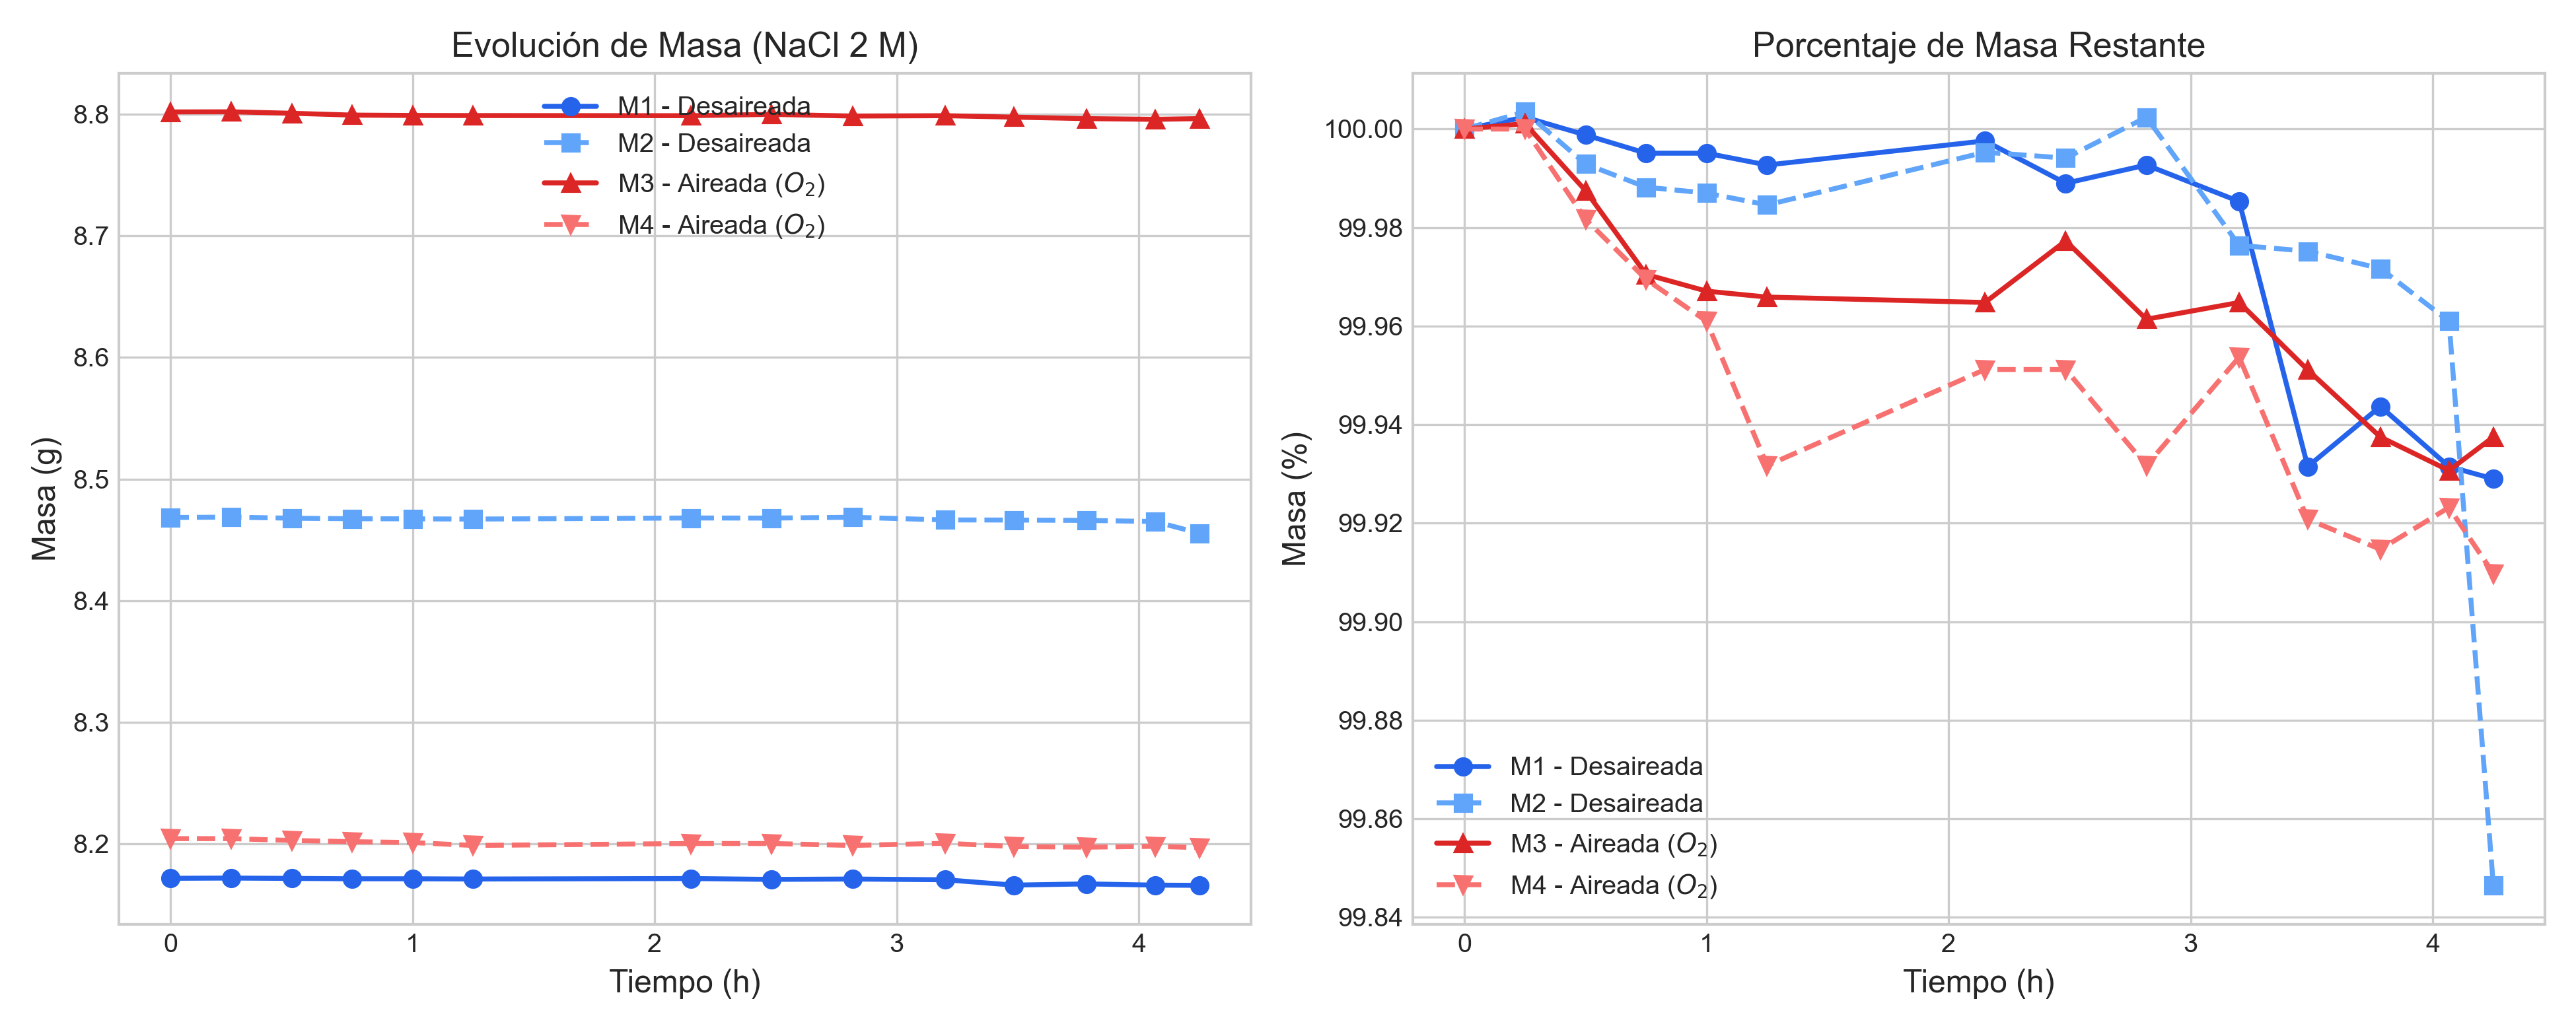
\includegraphics[width=0.92\textwidth]{resultados_practica_corrosion/exp_3_3_masa_y_pct.png}
    \caption{Evolución de masa (absoluta y en porcentaje) en función de la aireación del electrolito.}
    \label{fig:exp_3_3_masa}
\end{figure}

\begin{figure}[H]
    \centering
    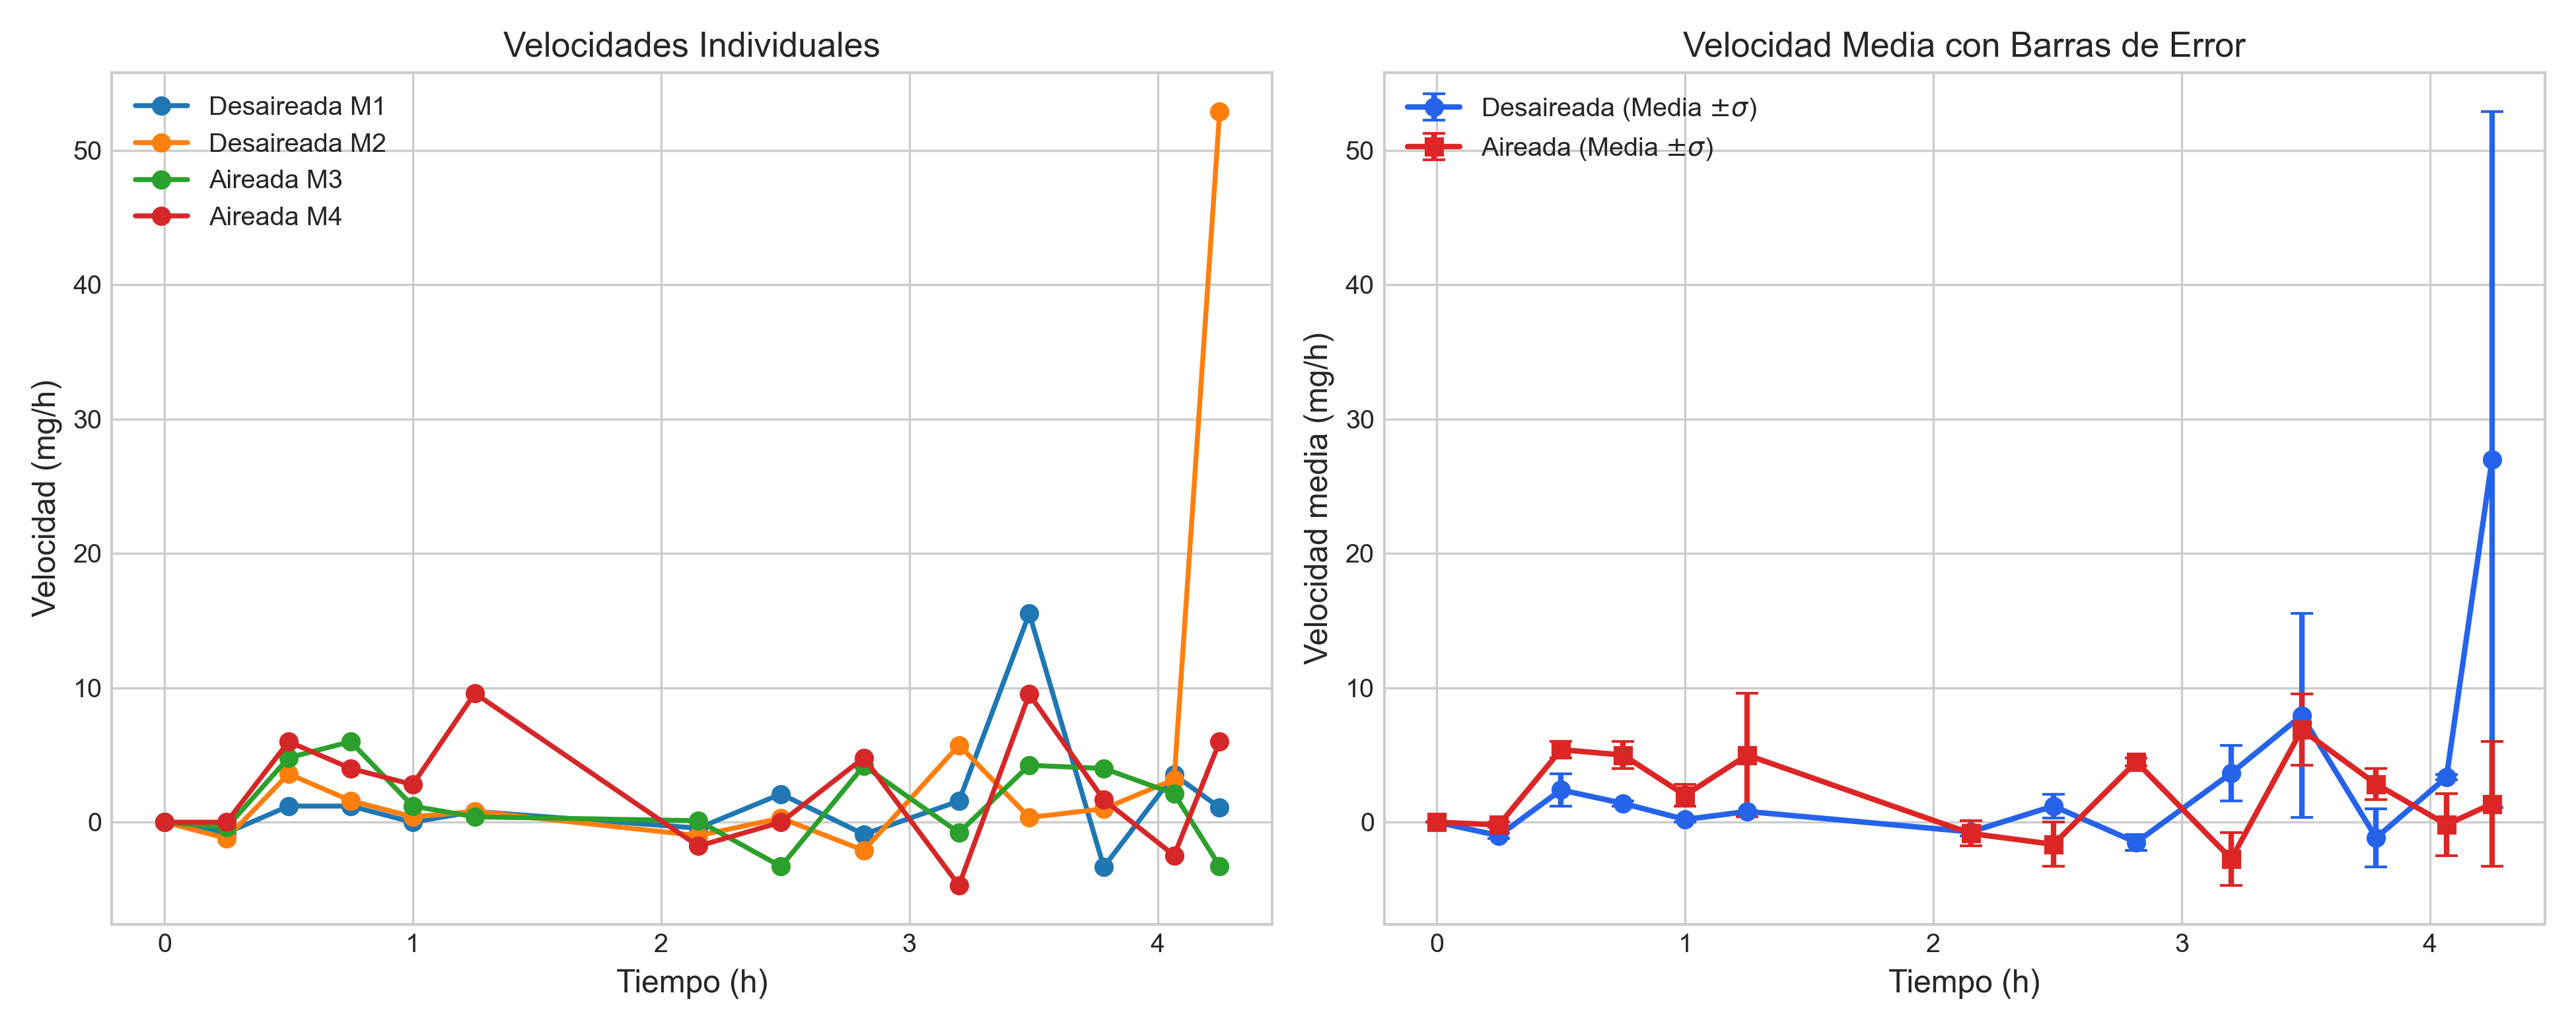
\includegraphics[width=0.92\textwidth]{resultados_practica_corrosion/exp_3_3_velocidad.png}
    \caption{Velocidades de corrosión individuales y velocidad media con barras de error (Desaireada vs Aireada).}
    \label{fig:exp_3_3_vel}
\end{figure}

% =============================================================================
\section{Experimento 3.4: Inhibición de la Corrosión por Productos Químicos (Subgrupo C)}
% =============================================================================
\subsection{Fundamento y Mecanismo del Fosfato Trisódico ($\text{Na}_3\text{PO}_4$)}
Los fosfatos actúan como \textbf{inhibidores anódicos pasivantes}. Al disociarse en medio acuoso ligeramente ácido/neutro:
\begin{align}
    \text{PO}_4^{3-} + \text{H}_2\text{O} &\rightleftharpoons \text{HPO}_4^{2-} + \text{OH}^- \\
    3\text{Fe}^{2+} + 2\text{PO}_4^{3-} &\longrightarrow \text{Fe}_3(\text{PO}_4)_2(\text{s}) \quad (K_{ps} \approx 10^{-33})
\end{align}
El fosfato ferroso precipita sobre las áreas anódicas activas, formando una película protectora impermeable que bloquea la transferencia de carga anódica.
\begin{itemize}
    \item Con $0\text{ mg/L}$: Se produce corrosión uniforme por aireación sin barrera pasivante.
    \item Con $2\text{ mg/L}$: Dosis insuficiente que puede producir pasivación incompleta (peligro de corrosión por picaduras si la relación catódica/anódica es desfavorable).
    \item Con $40\text{ mg/L}$: Concentración óptima que garantiza el cubrimiento superficial continuo, reduciendo drásticamente la tasa de corrosión global.
\end{itemize}

\subsection{Comentario sobre las Velocidades Negativas y Ganancia de Masa}
En las tablas se observan valores de velocidad negativos en ciertos intervalos puntuales (por ejemplo, a $t = 2.5\text{ h}$ o $t = 3.25\text{ h}$). Esto se debe a la formación de productos insolubles de corrosión ($\text{Fe(OH)}_2$, $\text{Fe}_3(\text{PO}_4)_2$ o herrumbre hidratada) que se adhieren a la superficie antes del lavado y secado, generando un ligero incremento temporal en el peso medido de la probeta.

\subsection{Resultados Experimentales y Gráficas}
\begin{table}[H]
\centering
\caption{Muestra 1 -- $[\text{Na}_3\text{PO}_4] = 0\text{ mg/L}$}
\label{tab:3_4_c0_m1}
\begin{tabular}{cccccc}
\toprule
t (min) & t (h) & Masa (g) & Masa (\%) & Pérdida (mg) & Velocidad (mg/h) \\
\midrule
0.0000 & 0.0000 & 8.2850 & 100.00 & 0.0000 & 0.0000 \\
10.0000 & 0.1667 & 8.2830 & 99.9759 & 2.0000 & 12.0000 \\
20.0000 & 0.3333 & 8.2817 & 99.9602 & 3.3000 & 7.8000 \\
30.0000 & 0.5000 & 8.2787 & 99.9240 & 6.3000 & 18.0000 \\
40.0000 & 0.6667 & 8.2780 & 99.9155 & 7.0000 & 4.2000 \\
60.0000 & 1.0000 & 8.2802 & 99.9421 & 4.8000 & -6.6000 \\
80.0000 & 1.3333 & 8.2808 & 99.9493 & 4.2000 & -1.8000 \\
100.00 & 1.6667 & 8.2799 & 99.9384 & 5.1000 & 2.7000 \\
120.00 & 2.0000 & 8.2810 & 99.9517 & 4.0000 & -3.3000 \\
140.00 & 2.3333 & 8.2794 & 99.9324 & 5.6000 & 4.8000 \\
150.00 & 2.5000 & 8.2994 & 100.17 & -14.4000 & -120.00 \\
165.00 & 2.7500 & 8.2990 & 100.17 & -14.0000 & 1.6000 \\
180.00 & 3.0000 & 8.2988 & 100.17 & -13.8000 & 0.8000 \\
195.00 & 3.2500 & 8.2993 & 100.17 & -14.3000 & -2.0000 \\
210.00 & 3.5000 & 8.2989 & 100.17 & -13.9000 & 1.6000 \\
225.00 & 3.7500 & 8.2993 & 100.17 & -14.3000 & -1.6000 \\
\bottomrule
\end{tabular}
\end{table}

\begin{table}[H]
\centering
\caption{Muestra 2 -- $[\text{Na}_3\text{PO}_4] = 0\text{ mg/L}$}
\label{tab:3_4_c0_m2}
\begin{tabular}{cccccc}
\toprule
t (min) & t (h) & Masa (g) & Masa (\%) & Pérdida (mg) & Velocidad (mg/h) \\
\midrule
0.0000 & 0.0000 & 8.7570 & 100.00 & 0.0000 & 0.0000 \\
10.0000 & 0.1667 & 8.7560 & 99.9886 & 1.0000 & 6.0000 \\
20.0000 & 0.3333 & 8.7534 & 99.9589 & 3.6000 & 15.6000 \\
30.0000 & 0.5000 & 8.7223 & 99.6037 & 34.7000 & 186.60 \\
40.0000 & 0.6667 & 8.7551 & 99.9783 & 1.9000 & -196.80 \\
60.0000 & 1.0000 & 8.7588 & 100.02 & -1.8000 & -11.1000 \\
80.0000 & 1.3333 & 8.7520 & 99.9429 & 5.0000 & 20.4000 \\
100.00 & 1.6667 & 8.7514 & 99.9361 & 5.6000 & 1.8000 \\
120.00 & 2.0000 & 8.7526 & 99.9498 & 4.4000 & -3.6000 \\
140.00 & 2.3333 & 8.7514 & 99.9361 & 5.6000 & 3.6000 \\
150.00 & 2.5000 & 8.7518 & 99.9406 & 5.2000 & -2.4000 \\
165.00 & 2.7500 & 8.7513 & 99.9349 & 5.7000 & 2.0000 \\
180.00 & 3.0000 & 8.7517 & 99.9395 & 5.3000 & -1.6000 \\
195.00 & 3.2500 & 8.7520 & 99.9429 & 5.0000 & -1.2000 \\
210.00 & 3.5000 & 8.7516 & 99.9383 & 5.4000 & 1.6000 \\
225.00 & 3.7500 & 8.7521 & 99.9440 & 4.9000 & -2.0000 \\
\bottomrule
\end{tabular}
\end{table}

\begin{table}[H]
\centering
\caption{Muestra 3 -- $[\text{Na}_3\text{PO}_4] = 2\text{ mg/L}$}
\label{tab:3_4_c2_m3}
\begin{tabular}{cccccc}
\toprule
t (min) & t (h) & Masa (g) & Masa (\%) & Pérdida (mg) & Velocidad (mg/h) \\
\midrule
0.0000 & 0.0000 & 8.3000 & 100.00 & 0.0000 & 0.0000 \\
10.0000 & 0.1667 & 8.2970 & 99.9639 & 3.0000 & 18.0000 \\
20.0000 & 0.3333 & 8.2930 & 99.9157 & 7.0000 & 24.0000 \\
30.0000 & 0.5000 & 8.2900 & 99.8795 & 10.0000 & 18.0000 \\
40.0000 & 0.6667 & 8.2980 & 99.9759 & 2.0000 & -48.0000 \\
60.0000 & 1.0000 & 8.2996 & 99.9952 & 0.4000 & -4.8000 \\
80.0000 & 1.3333 & 8.2989 & 99.9867 & 1.1000 & 2.1000 \\
100.00 & 1.6667 & 8.2992 & 99.9904 & 0.8000 & -0.9000 \\
120.00 & 2.0000 & 8.2989 & 99.9867 & 1.1000 & 0.9000 \\
140.00 & 2.3333 & 8.2983 & 99.9795 & 1.7000 & 1.8000 \\
150.00 & 2.5000 & 8.2790 & 99.7470 & 21.0000 & 115.80 \\
165.00 & 2.7500 & 8.2790 & 99.7470 & 21.0000 & -0.0000 \\
180.00 & 3.0000 & 8.2795 & 99.7530 & 20.5000 & -2.0000 \\
195.00 & 3.2500 & 8.2784 & 99.7398 & 21.6000 & 4.4000 \\
210.00 & 3.5000 & 8.2801 & 99.7602 & 19.9000 & -6.8000 \\
225.00 & 3.7500 & 8.2794 & 99.7518 & 20.6000 & 2.8000 \\
\bottomrule
\end{tabular}
\end{table}

\begin{table}[H]
\centering
\caption{Muestra 4 -- $[\text{Na}_3\text{PO}_4] = 2\text{ mg/L}$}
\label{tab:3_4_c2_m4}
\begin{tabular}{cccccc}
\toprule
t (min) & t (h) & Masa (g) & Masa (\%) & Pérdida (mg) & Velocidad (mg/h) \\
\midrule
0.0000 & 0.0000 & 8.7840 & 100.00 & 0.0000 & 0.0000 \\
10.0000 & 0.1667 & 8.7420 & 99.5219 & 42.0000 & 252.00 \\
20.0000 & 0.3333 & 8.7420 & 99.5219 & 42.0000 & -0.0000 \\
30.0000 & 0.5000 & 8.7420 & 99.5219 & 42.0000 & -0.0000 \\
40.0000 & 0.6667 & 8.7420 & 99.5219 & 42.0000 & -0.0000 \\
60.0000 & 1.0000 & 8.7421 & 99.5230 & 41.9000 & -0.3000 \\
80.0000 & 1.3333 & 8.7410 & 99.5105 & 43.0000 & 3.3000 \\
100.00 & 1.6667 & 8.7414 & 99.5150 & 42.6000 & -1.2000 \\
120.00 & 2.0000 & 8.7407 & 99.5071 & 43.3000 & 2.1000 \\
140.00 & 2.3333 & 8.7412 & 99.5128 & 42.8000 & -1.5000 \\
150.00 & 2.5000 & 8.6758 & 98.7682 & 108.20 & 392.40 \\
165.00 & 2.7500 & 8.6757 & 98.7671 & 108.30 & 0.4000 \\
180.00 & 3.0000 & 8.6764 & 98.7750 & 107.60 & -2.8000 \\
195.00 & 3.2500 & 8.6770 & 98.7819 & 107.00 & -2.4000 \\
210.00 & 3.5000 & 8.6757 & 98.7671 & 108.30 & 5.2000 \\
225.00 & 3.7500 & 8.6758 & 98.7682 & 108.20 & -0.4000 \\
\bottomrule
\end{tabular}
\end{table}

\begin{table}[H]
\centering
\caption{Muestra 5 -- $[\text{Na}_3\text{PO}_4] = 40\text{ mg/L}$}
\label{tab:3_4_c40_m5}
\begin{tabular}{cccccc}
\toprule
t (min) & t (h) & Masa (g) & Masa (\%) & Pérdida (mg) & Velocidad (mg/h) \\
\midrule
0.0000 & 0.0000 & 8.6790 & 100.00 & 0.0000 & 0.0000 \\
10.0000 & 0.1667 & 8.6790 & 100.00 & 0.0000 & -0.0000 \\
20.0000 & 0.3333 & 8.6780 & 99.9885 & 1.0000 & 6.0000 \\
30.0000 & 0.5000 & 8.6787 & 99.9965 & 0.3000 & -4.2000 \\
40.0000 & 0.6667 & 8.6760 & 99.9654 & 3.0000 & 16.2000 \\
60.0000 & 1.0000 & 8.6764 & 99.9700 & 2.6000 & -1.2000 \\
80.0000 & 1.3333 & 8.6762 & 99.9677 & 2.8000 & 0.6000 \\
100.00 & 1.6667 & 8.6761 & 99.9666 & 2.9000 & 0.3000 \\
120.00 & 2.0000 & 8.6771 & 99.9781 & 1.9000 & -3.0000 \\
140.00 & 2.3333 & 8.6763 & 99.9689 & 2.7000 & 2.4000 \\
150.00 & 2.5000 & 8.6758 & 99.9631 & 3.2000 & 3.0000 \\
165.00 & 2.7500 & 8.6757 & 99.9620 & 3.3000 & 0.4000 \\
180.00 & 3.0000 & 8.6764 & 99.9700 & 2.6000 & -2.8000 \\
195.00 & 3.2500 & 8.6770 & 99.9770 & 2.0000 & -2.4000 \\
210.00 & 3.5000 & 8.6757 & 99.9620 & 3.3000 & 5.2000 \\
225.00 & 3.7500 & 8.6758 & 99.9631 & 3.2000 & -0.4000 \\
\bottomrule
\end{tabular}
\end{table}

\begin{table}[H]
\centering
\caption{Muestra 6 -- $[\text{Na}_3\text{PO}_4] = 40\text{ mg/L}$}
\label{tab:3_4_c40_m6}
\begin{tabular}{cccccc}
\toprule
t (min) & t (h) & Masa (g) & Masa (\%) & Pérdida (mg) & Velocidad (mg/h) \\
\midrule
0.0000 & 0.0000 & 8.1990 & 100.00 & 0.0000 & 0.0000 \\
10.0000 & 0.1667 & 8.1990 & 100.00 & 0.0000 & -0.0000 \\
20.0000 & 0.3333 & 8.1909 & 99.9012 & 8.1000 & 48.6000 \\
30.0000 & 0.5000 & 8.1910 & 99.9024 & 8.0000 & -0.6000 \\
40.0000 & 0.6667 & 8.1880 & 99.8658 & 11.0000 & 18.0000 \\
60.0000 & 1.0000 & 8.1893 & 99.8817 & 9.7000 & -3.9000 \\
80.0000 & 1.3333 & 8.1893 & 99.8817 & 9.7000 & -0.0000 \\
100.00 & 1.6667 & 8.1895 & 99.8841 & 9.5000 & -0.6000 \\
120.00 & 2.0000 & 8.1902 & 99.8927 & 8.8000 & -2.1000 \\
140.00 & 2.3333 & 8.1903 & 99.8939 & 8.7000 & -0.3000 \\
150.00 & 2.5000 & 8.1890 & 99.8780 & 10.0000 & 7.8000 \\
165.00 & 2.7500 & 8.1926 & 99.9219 & 6.4000 & -14.4000 \\
180.00 & 3.0000 & 8.1898 & 99.8878 & 9.2000 & 11.2000 \\
195.00 & 3.2500 & 8.1896 & 99.8854 & 9.4000 & 0.8000 \\
210.00 & 3.5000 & 8.1902 & 99.8927 & 8.8000 & -2.4000 \\
225.00 & 3.7500 & 8.1901 & 99.8915 & 8.9000 & 0.4000 \\
\bottomrule
\end{tabular}
\end{table}


\begin{figure}[H]
    \centering
    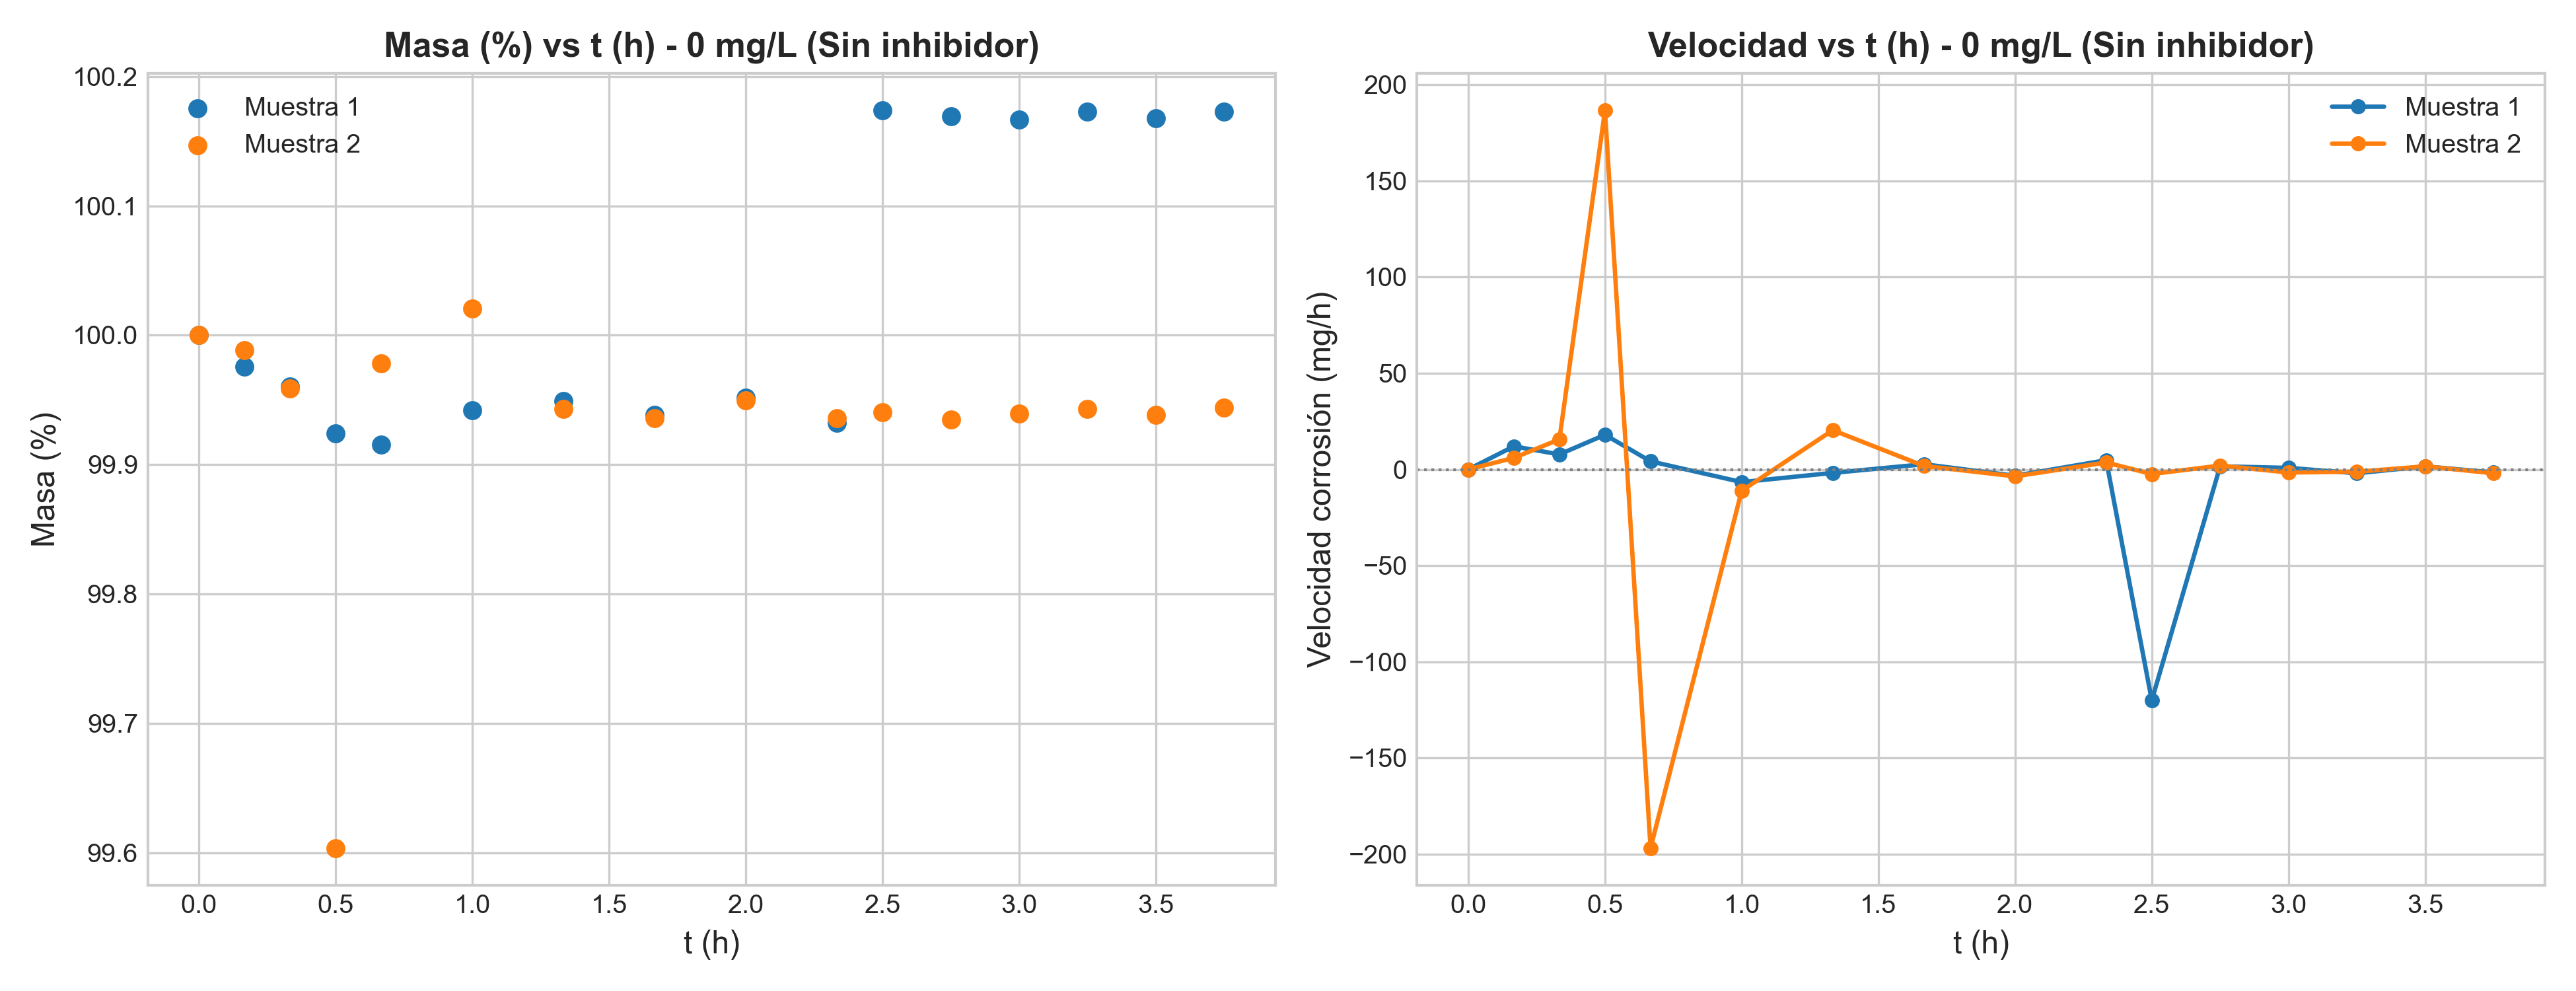
\includegraphics[width=0.95\textwidth]{resultados_practica_corrosion/exp_3_4_individual_0mgL.png}
    \caption{Evolución de Masa (\%) vs $t$ y Velocidad vs $t$ para $[\text{Na}_3\text{PO}_4] = 0\text{ mg/L}$ (Muestra 1 y Muestra 2).}
    \label{fig:exp_3_4_0mgL}
\end{figure}

\begin{figure}[H]
    \centering
    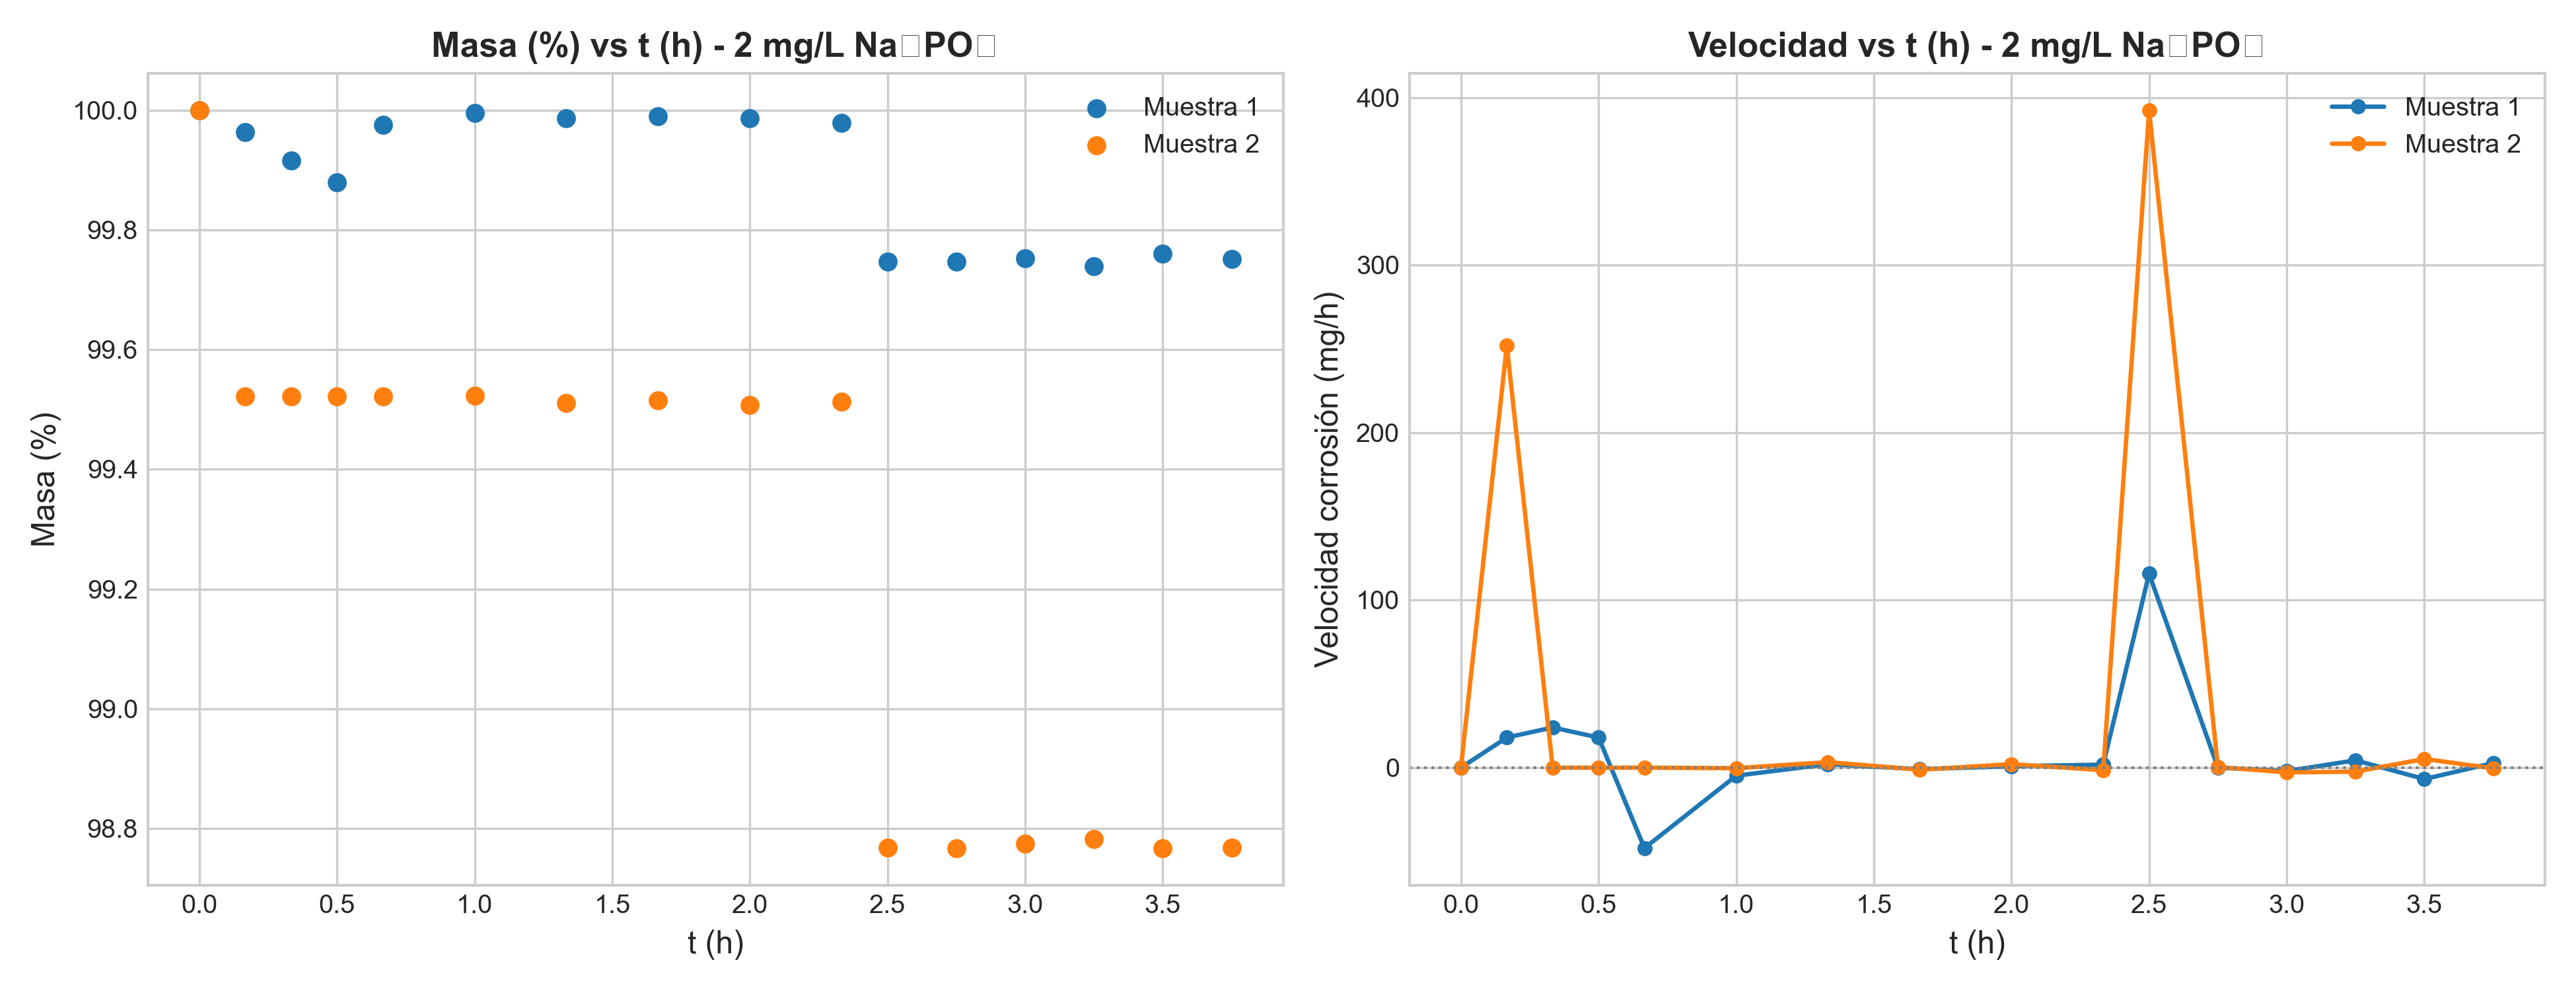
\includegraphics[width=0.95\textwidth]{resultados_practica_corrosion/exp_3_4_individual_2mgL.png}
    \caption{Evolución de Masa (\%) vs $t$ y Velocidad vs $t$ para $[\text{Na}_3\text{PO}_4] = 2\text{ mg/L}$ (Muestra 3 y Muestra 4).}
    \label{fig:exp_3_4_2mgL}
\end{figure}

\begin{figure}[H]
    \centering
    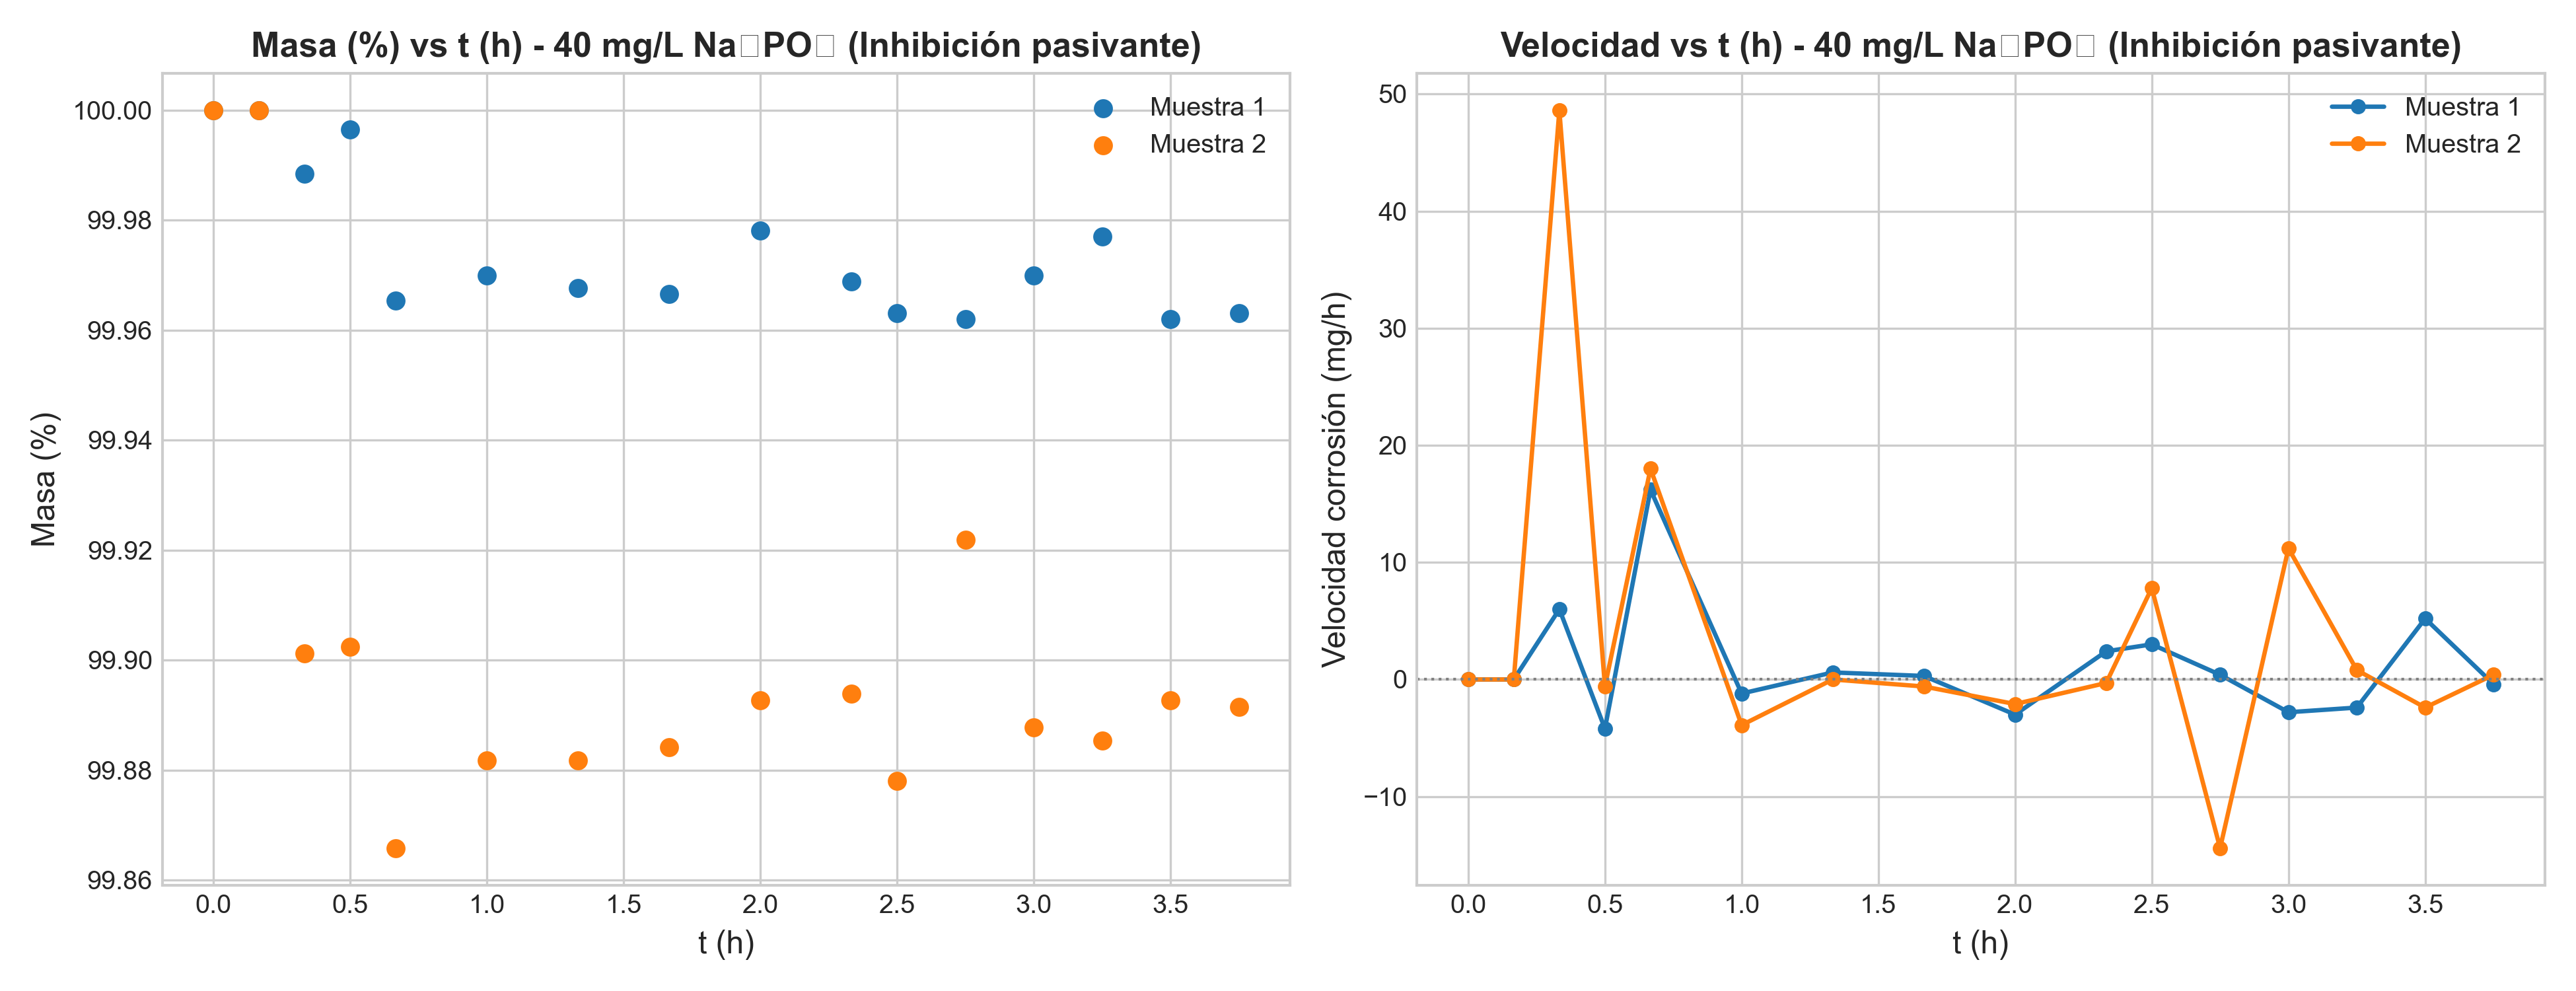
\includegraphics[width=0.95\textwidth]{resultados_practica_corrosion/exp_3_4_individual_40mgL.png}
    \caption{Evolución de Masa (\%) vs $t$ y Velocidad vs $t$ para $[\text{Na}_3\text{PO}_4] = 40\text{ mg/L}$ (Muestra 5 y Muestra 6).}
    \label{fig:exp_3_4_40mgL}
\end{figure}

\begin{figure}[H]
    \centering
    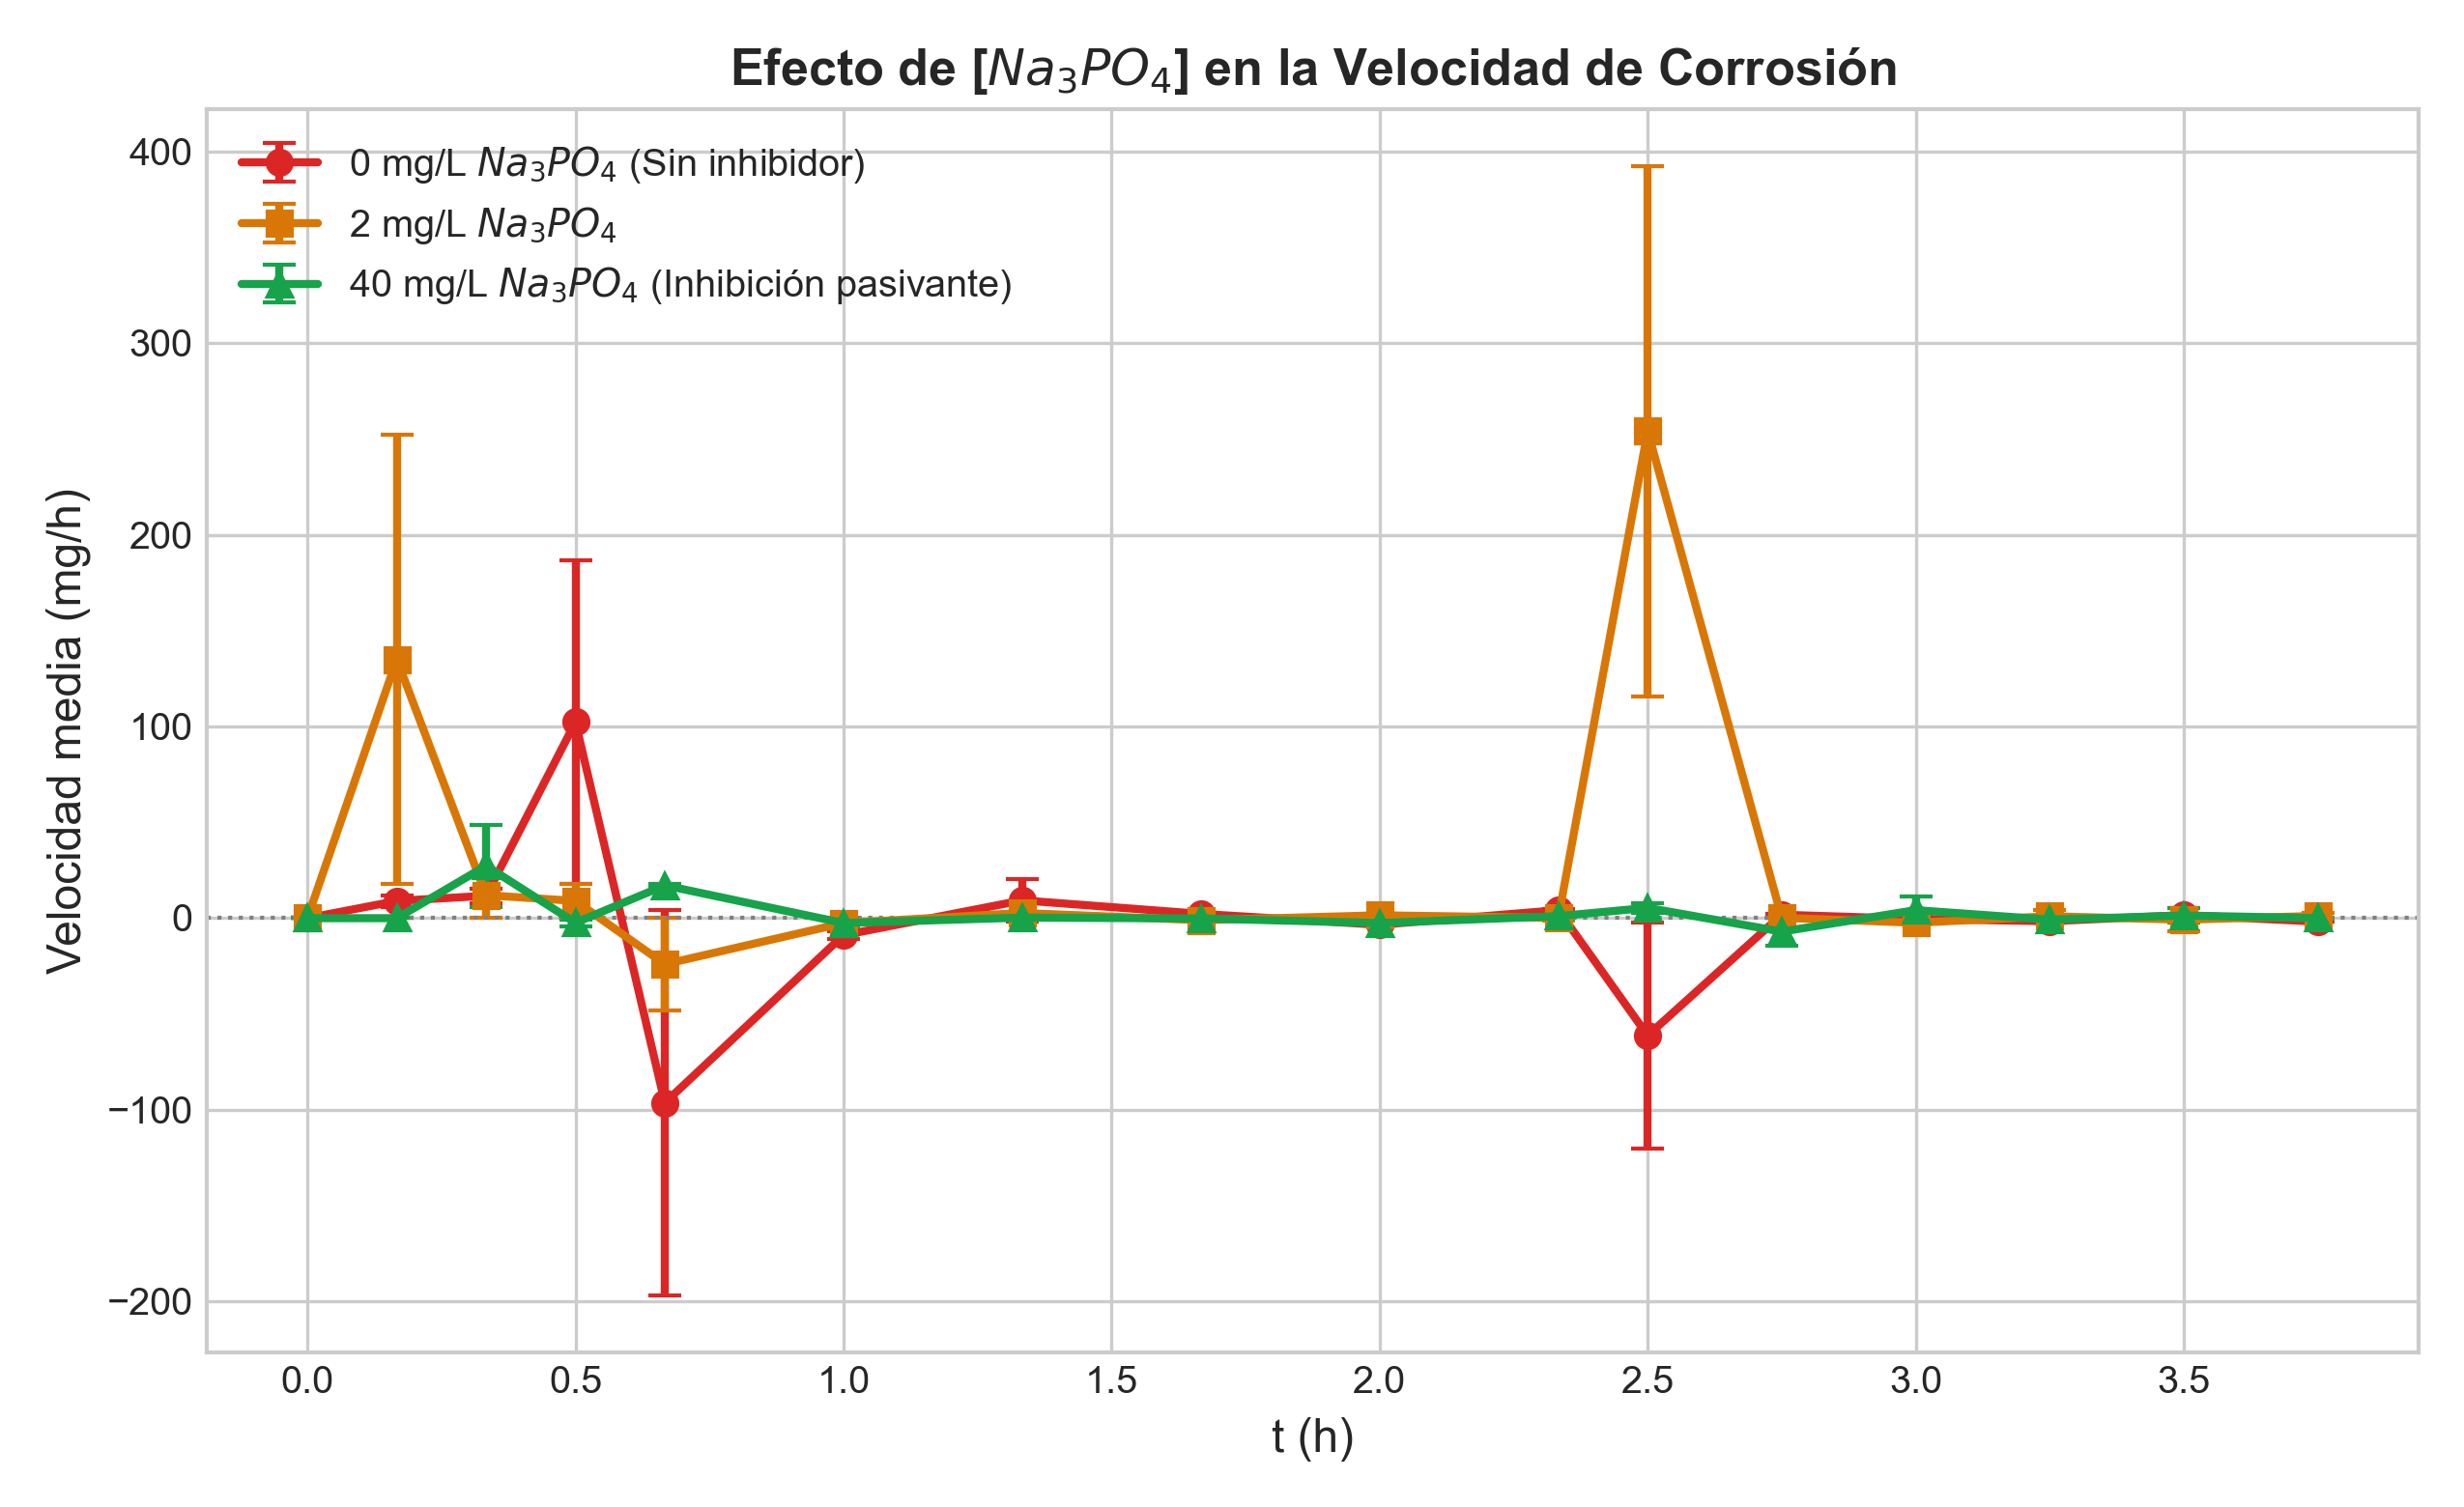
\includegraphics[width=0.82\textwidth]{resultados_practica_corrosion/exp_3_4_comparativa_global.png}
    \caption{Comparativa global de la velocidad media de corrosión con barras de error para las tres concentraciones de inhibidor.}
    \label{fig:exp_3_4_comp}
\end{figure}

% =============================================================================
\section{Experimento 3.5: Protección Catódica por Corriente Impresa}
% =============================================================================
\subsection{Fundamento y Esquema Experimental}
La protección catódica por corriente impresa (ICCP) consiste en suministrar electrones desde una fuente externa de corriente continua para desplazar el potencial del metal a proteger hacia su \textbf{zona de inmunidad termodinámica} según el Diagrama de Pourbaix.

En una disolución fuertemente alcalina ($\text{NaOH}$ pH 13 con $\text{KCl}$ $4.1\text{ g/L}$ para máxima conductividad) y aplicando $10\text{ V}$:
\begin{itemize}
    \item \textbf{Cátodo (Polo Negativo -- Probeta Protegida)}:
    \begin{equation}
        2\text{H}_2\text{O} + 2e^- \longrightarrow \text{H}_2(\text{g}) \uparrow + 2\text{OH}^- \quad (E = -0.0591 \cdot \text{pH} = -0.768\text{ V vs SHE})
    \end{equation}
    Se observa un intenso desprendimiento de burbujas de hidrógeno molecular ($\text{H}_2$). El metal se mantiene inalterado, brillante y libre de corrosión gracias a la sobretensión catódica.
    \item \textbf{Ánodo Auxiliar (Polo Positivo)}:
    \begin{equation}
        4\text{OH}^- \longrightarrow \text{O}_2(\text{g}) \uparrow + 2\text{H}_2\text{O} + 4e^- \quad \text{y/o} \quad \text{Fe} \longrightarrow \text{Fe}^{2+} + 2e^-
    \end{equation}
    Se produce desprendimiento de oxígeno y ataque electroquímico anódico acelerado.
\end{itemize}

\begin{figure}[H]
    \centering
    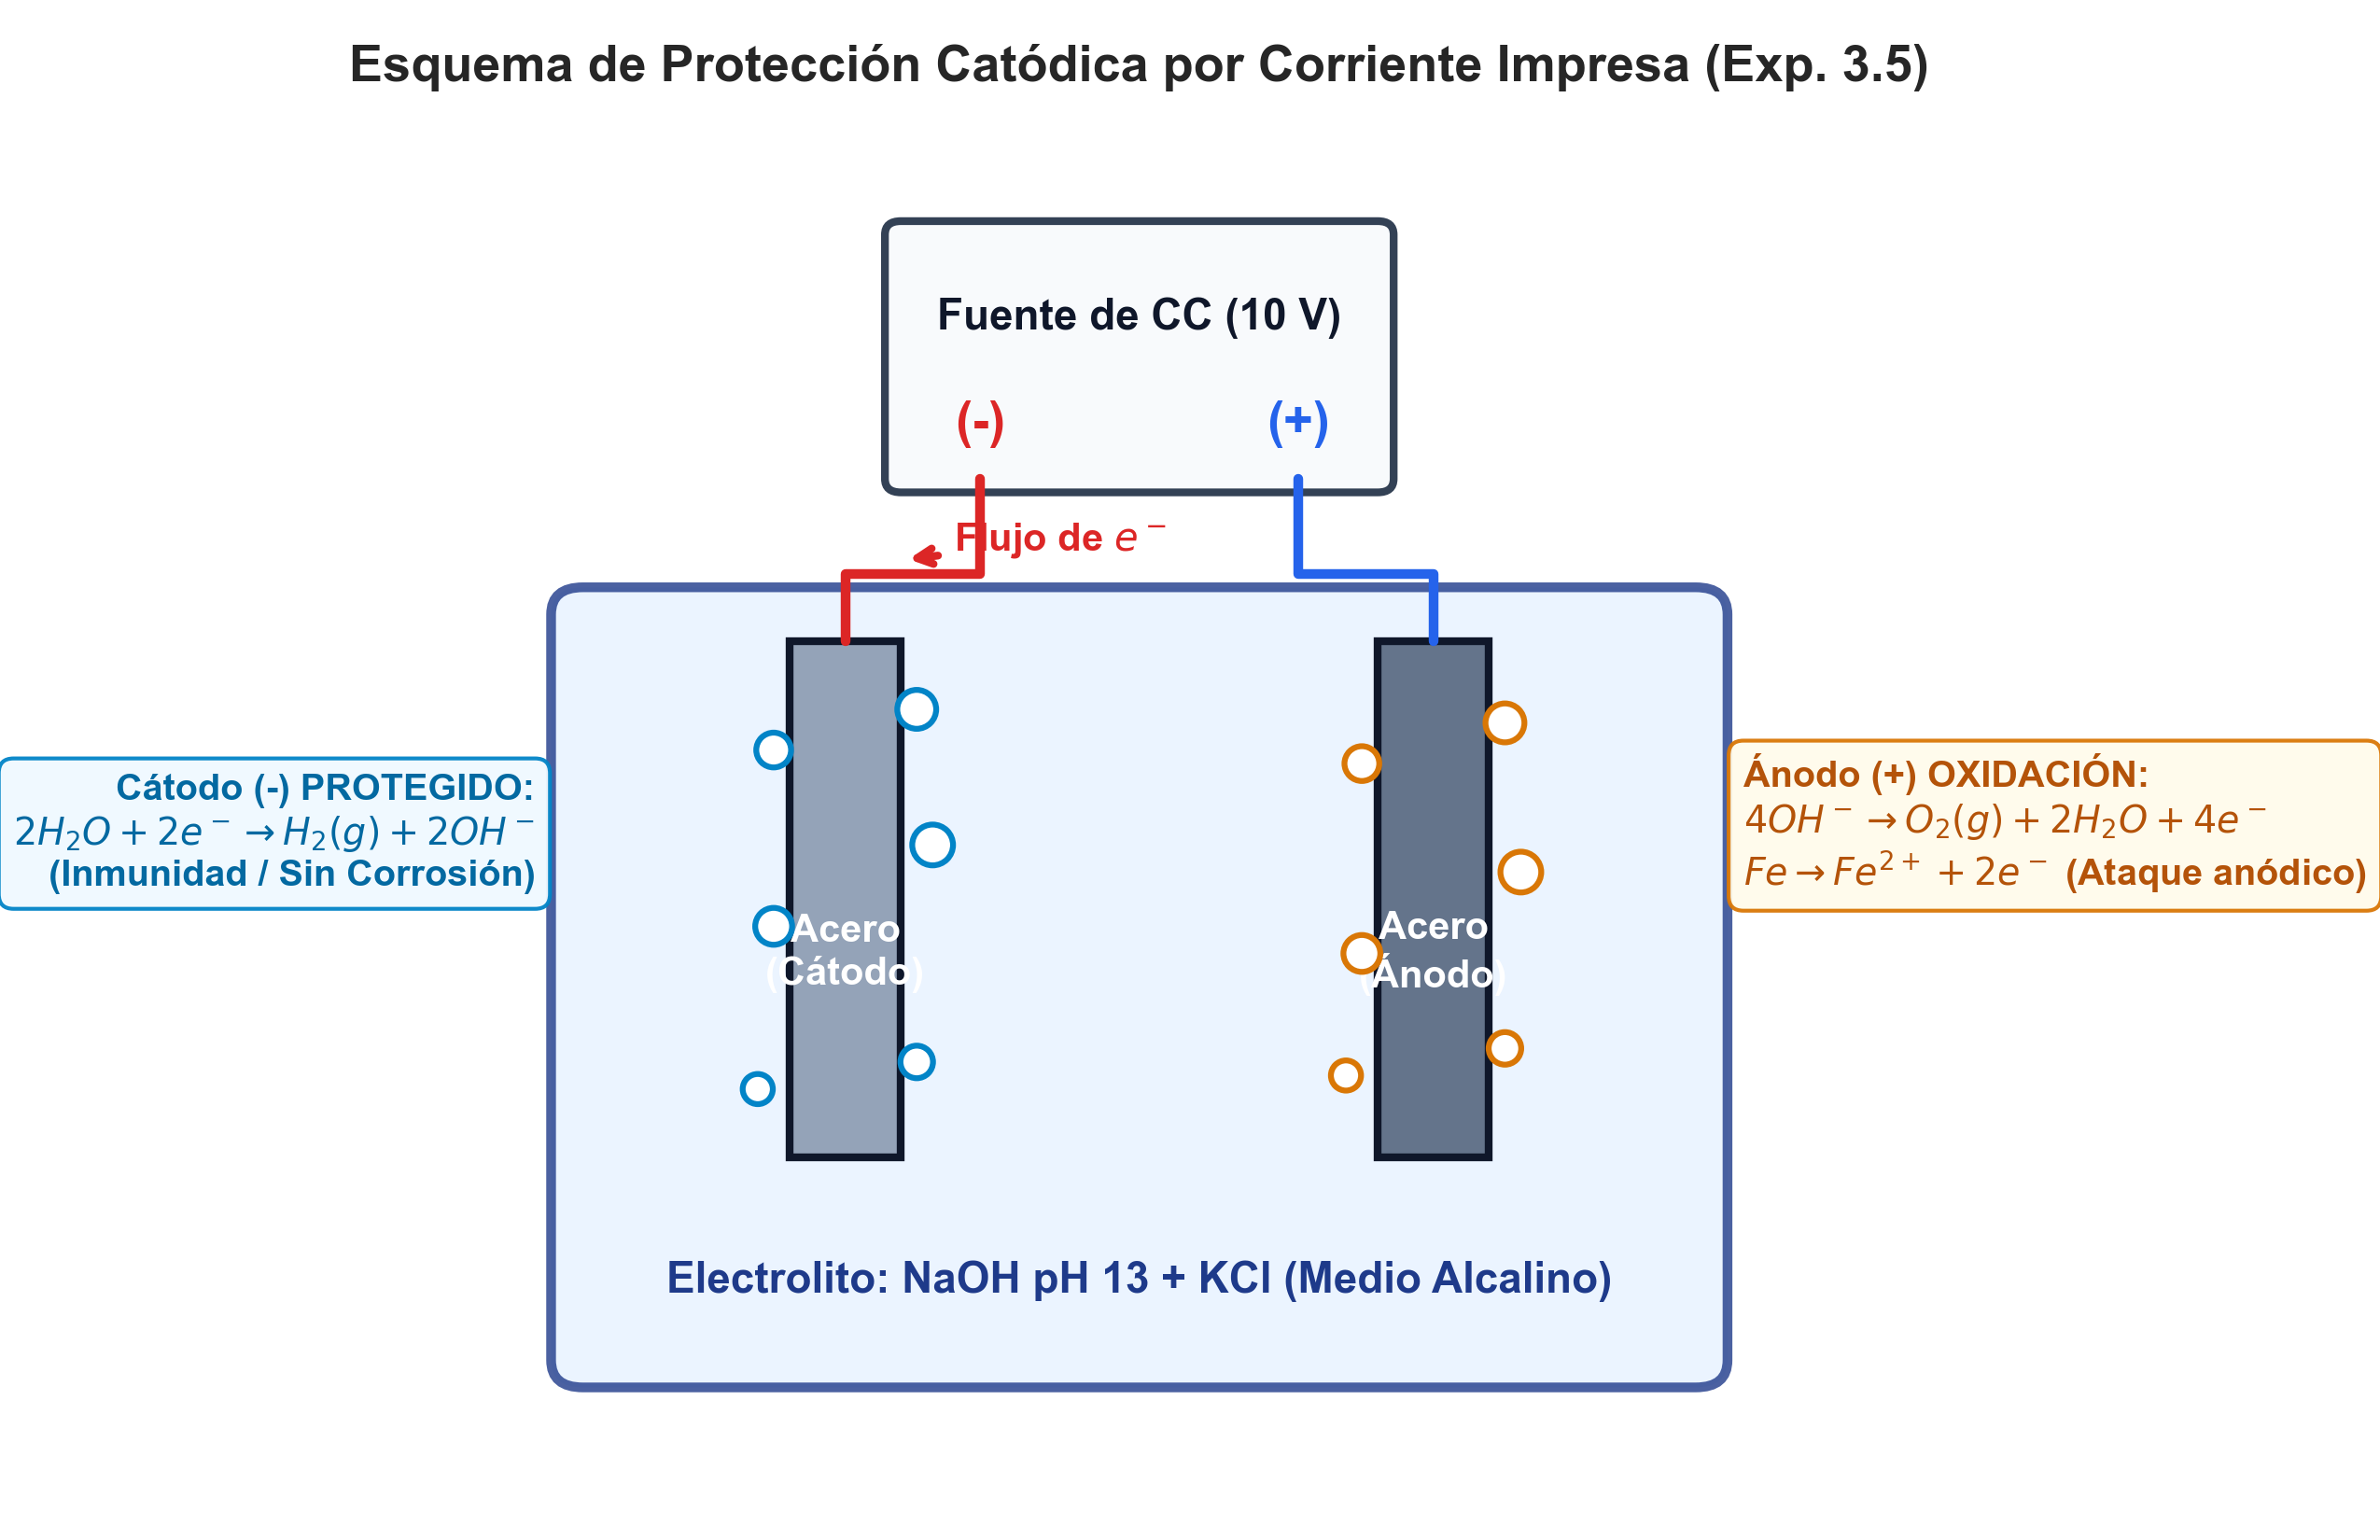
\includegraphics[width=0.85\textwidth]{resultados_practica_corrosion/exp_3_5_esquema_proteccion_catodica.png}
    \caption{Esquema de celda de protección catódica por corriente impresa con reacciones electrolíticas.}
    \label{fig:exp_3_5_esquema}
\end{figure}

% =============================================================================
\section{Experimento 3.6: Corrosión Galvánica (Subgrupo D)}
% =============================================================================
\subsection{Fundamento y Serie Galvánica}
Al unir eléctricamente dos metales distintos en un electrolito conductor:
\begin{itemize}
    \item El metal con potencial estándar más electronegativo actúa como \textbf{ánodo de sacrificio} y se disuelve preferencialmente.
    \item El metal con potencial más noble actúa como \textbf{cátodo}, recibiendo electrones y reduciendo su tasa de degradación.
\end{itemize}

\subsubsection{Par 1: Acero -- Zinc ($\text{Acero}-\text{Zn}$)}
Potenciales estándar: $E^0_{\text{Zn}^{2+}/\text{Zn}} = -0.763\text{ V} < E^0_{\text{Fe}^{2+}/\text{Fe}} = -0.44\text{ V}$.
\begin{align}
    \text{Ánodo (Zinc sacrificado):} \quad & \text{Zn} \longrightarrow \text{Zn}^{2+} + 2e^- \\
    \text{Cátodo (Acero protegido):} \quad & \text{O}_2 + 2\text{H}_2\text{O} + 4e^- \longrightarrow 4\text{OH}^-
\end{align}
El zinc sufre una disolución acelerada protegiendo íntegramente al acero.

\subsubsection{Par 2: Acero -- Cobre ($\text{Acero}-\text{Cu}$)}
Potenciales estándar: $E^0_{\text{Fe}^{2+}/\text{Fe}} = -0.44\text{ V} < E^0_{\text{Cu}^{2+}/\text{Cu}} = +0.34\text{ V}$.
\begin{align}
    \text{Ánodo (Acero corroído aceleradamente):} \quad & \text{Fe} \longrightarrow \text{Fe}^{2+} + 2e^- \\
    \text{Cátodo (Cobre intacto):} \quad & \text{O}_2 + 2\text{H}_2\text{O} + 4e^- \longrightarrow 4\text{OH}^-
\end{align}
El cobre incrementa drásticamente la densidad de corriente anódica en el acero, induciendo una severa corrosión galvánica.

\subsection{Resultados Experimentales y Gráficas}
\begin{table}[H]
\centering
\caption{Par Galvánico 1: Acero 1 (Cátodo protegido por Zn)}
\label{tab:3_6_acero1}
\begin{tabular}{cccccc}
\toprule
t (min) & t (h) & Masa (g) & Masa (\%) & Pérdida (mg) & Velocidad (mg/h) \\
\midrule
0.0000 & 0.0000 & 8.6991 & 100.00 & 0.0000 & 0.0000 \\
10.0000 & 0.1667 & 8.6996 & 100.01 & -0.5000 & -3.0000 \\
20.0000 & 0.3333 & 8.7002 & 100.01 & -1.1000 & -3.6000 \\
35.0000 & 0.5833 & 8.6986 & 99.9943 & 0.5000 & 6.4000 \\
50.0000 & 0.8333 & 8.6959 & 99.9632 & 3.2000 & 10.8000 \\
75.0000 & 1.2500 & 8.7002 & 100.01 & -1.1000 & -10.3200 \\
90.0000 & 1.5000 & 8.7002 & 100.01 & -1.1000 & -0.0000 \\
110.00 & 1.8333 & 8.6984 & 99.9920 & 0.7000 & 5.4000 \\
130.00 & 2.1667 & 8.6990 & 99.9989 & 0.1000 & -1.8000 \\
150.00 & 2.5000 & 8.6985 & 99.9931 & 0.6000 & 1.5000 \\
170.00 & 2.8333 & 8.7000 & 100.01 & -0.9000 & -4.5000 \\
190.00 & 3.1667 & 8.6996 & 100.01 & -0.5000 & 1.2000 \\
210.00 & 3.5000 & 8.6996 & 100.01 & -0.5000 & -0.0000 \\
230.00 & 3.8333 & 8.6982 & 99.9897 & 0.9000 & 4.2000 \\
\bottomrule
\end{tabular}
\end{table}

\begin{table}[H]
\centering
\caption{Par Galvánico 1: Zinc (Ánodo de sacrificio frente al acero)}
\label{tab:3_6_zn}
\begin{tabular}{cccccc}
\toprule
t (min) & t (h) & Masa (g) & Masa (\%) & Pérdida (mg) & Velocidad (mg/h) \\
\midrule
0.0000 & 0.0000 & 7.9930 & 100.00 & 0.0000 & 0.0000 \\
10.0000 & 0.1667 & 7.9968 & 100.05 & -3.8000 & -22.8000 \\
20.0000 & 0.3333 & 7.9953 & 100.03 & -2.3000 & 9.0000 \\
35.0000 & 0.5833 & 7.9956 & 100.03 & -2.6000 & -1.2000 \\
50.0000 & 0.8333 & 7.9952 & 100.03 & -2.2000 & 1.6000 \\
75.0000 & 1.2500 & 7.9947 & 100.02 & -1.7000 & 1.2000 \\
90.0000 & 1.5000 & 7.7916 & 97.4803 & 201.40 & 812.40 \\
110.00 & 1.8333 & 7.7918 & 97.4828 & 201.20 & -0.6000 \\
130.00 & 2.1667 & 7.7912 & 97.4753 & 201.80 & 1.8000 \\
150.00 & 2.5000 & 7.7917 & 97.4815 & 201.30 & -1.5000 \\
170.00 & 2.8333 & 7.7921 & 97.4866 & 200.90 & -1.2000 \\
190.00 & 3.1667 & 7.7922 & 97.4878 & 200.80 & -0.3000 \\
210.00 & 3.5000 & 7.7905 & 97.4665 & 202.50 & 5.1000 \\
230.00 & 3.8333 & 7.7918 & 97.4828 & 201.20 & -3.9000 \\
\bottomrule
\end{tabular}
\end{table}

\begin{table}[H]
\centering
\caption{Par Galvánico 2: Acero 2 (Ánodo activo frente al Cu)}
\label{tab:3_6_acero2}
\begin{tabular}{cccccc}
\toprule
t (min) & t (h) & Masa (g) & Masa (\%) & Pérdida (mg) & Velocidad (mg/h) \\
\midrule
0.0000 & 0.0000 & 7.7931 & 100.00 & 0.0000 & 0.0000 \\
10.0000 & 0.1667 & 7.7924 & 99.9910 & 0.7000 & 4.2000 \\
20.0000 & 0.3333 & 7.7904 & 99.9654 & 2.7000 & 12.0000 \\
35.0000 & 0.5833 & 7.7925 & 99.9923 & 0.6000 & -8.4000 \\
50.0000 & 0.8333 & 7.7928 & 99.9962 & 0.3000 & -1.2000 \\
75.0000 & 1.2500 & 7.7931 & 100.00 & 0.0000 & -0.7200 \\
90.0000 & 1.5000 & 7.9916 & 102.55 & -198.50 & -794.00 \\
110.00 & 1.8333 & 7.9922 & 102.55 & -199.10 & -1.8000 \\
130.00 & 2.1667 & 7.9933 & 102.57 & -200.20 & -3.3000 \\
150.00 & 2.5000 & 7.9937 & 102.57 & -200.60 & -1.2000 \\
170.00 & 2.8333 & 8.0040 & 102.71 & -210.90 & -30.9000 \\
190.00 & 3.1667 & 7.9927 & 102.56 & -199.60 & 33.9000 \\
210.00 & 3.5000 & 7.9922 & 102.55 & -199.10 & 1.5000 \\
230.00 & 3.8333 & 7.9920 & 102.55 & -198.90 & 0.6000 \\
\bottomrule
\end{tabular}
\end{table}

\begin{table}[H]
\centering
\caption{Par Galvánico 2: Cobre (Cátodo noble frente al acero)}
\label{tab:3_6_cu}
\begin{tabular}{cccccc}
\toprule
t (min) & t (h) & Masa (g) & Masa (\%) & Pérdida (mg) & Velocidad (mg/h) \\
\midrule
0.0000 & 0.0000 & 9.6541 & 100.00 & 0.0000 & 0.0000 \\
10.0000 & 0.1667 & 9.6534 & 99.9927 & 0.7000 & 4.2000 \\
20.0000 & 0.3333 & 9.6538 & 99.9969 & 0.3000 & -2.4000 \\
35.0000 & 0.5833 & 9.6537 & 99.9959 & 0.4000 & 0.4000 \\
50.0000 & 0.8333 & 9.6537 & 99.9959 & 0.4000 & -0.0000 \\
75.0000 & 1.2500 & 9.6531 & 99.9896 & 1.0000 & 1.4400 \\
90.0000 & 1.5000 & 9.6526 & 99.9845 & 1.5000 & 2.0000 \\
110.00 & 1.8333 & 9.6500 & 99.9575 & 4.1000 & 7.8000 \\
130.00 & 2.1667 & 9.6508 & 99.9658 & 3.3000 & -2.4000 \\
150.00 & 2.5000 & 9.6507 & 99.9648 & 3.4000 & 0.3000 \\
170.00 & 2.8333 & 9.6504 & 99.9617 & 3.7000 & 0.9000 \\
190.00 & 3.1667 & 9.6507 & 99.9648 & 3.4000 & -0.9000 \\
210.00 & 3.5000 & 9.6512 & 99.9700 & 2.9000 & -1.5000 \\
230.00 & 3.8333 & 9.6503 & 99.9606 & 3.8000 & 2.7000 \\
\bottomrule
\end{tabular}
\end{table}


\begin{figure}[H]
    \centering
    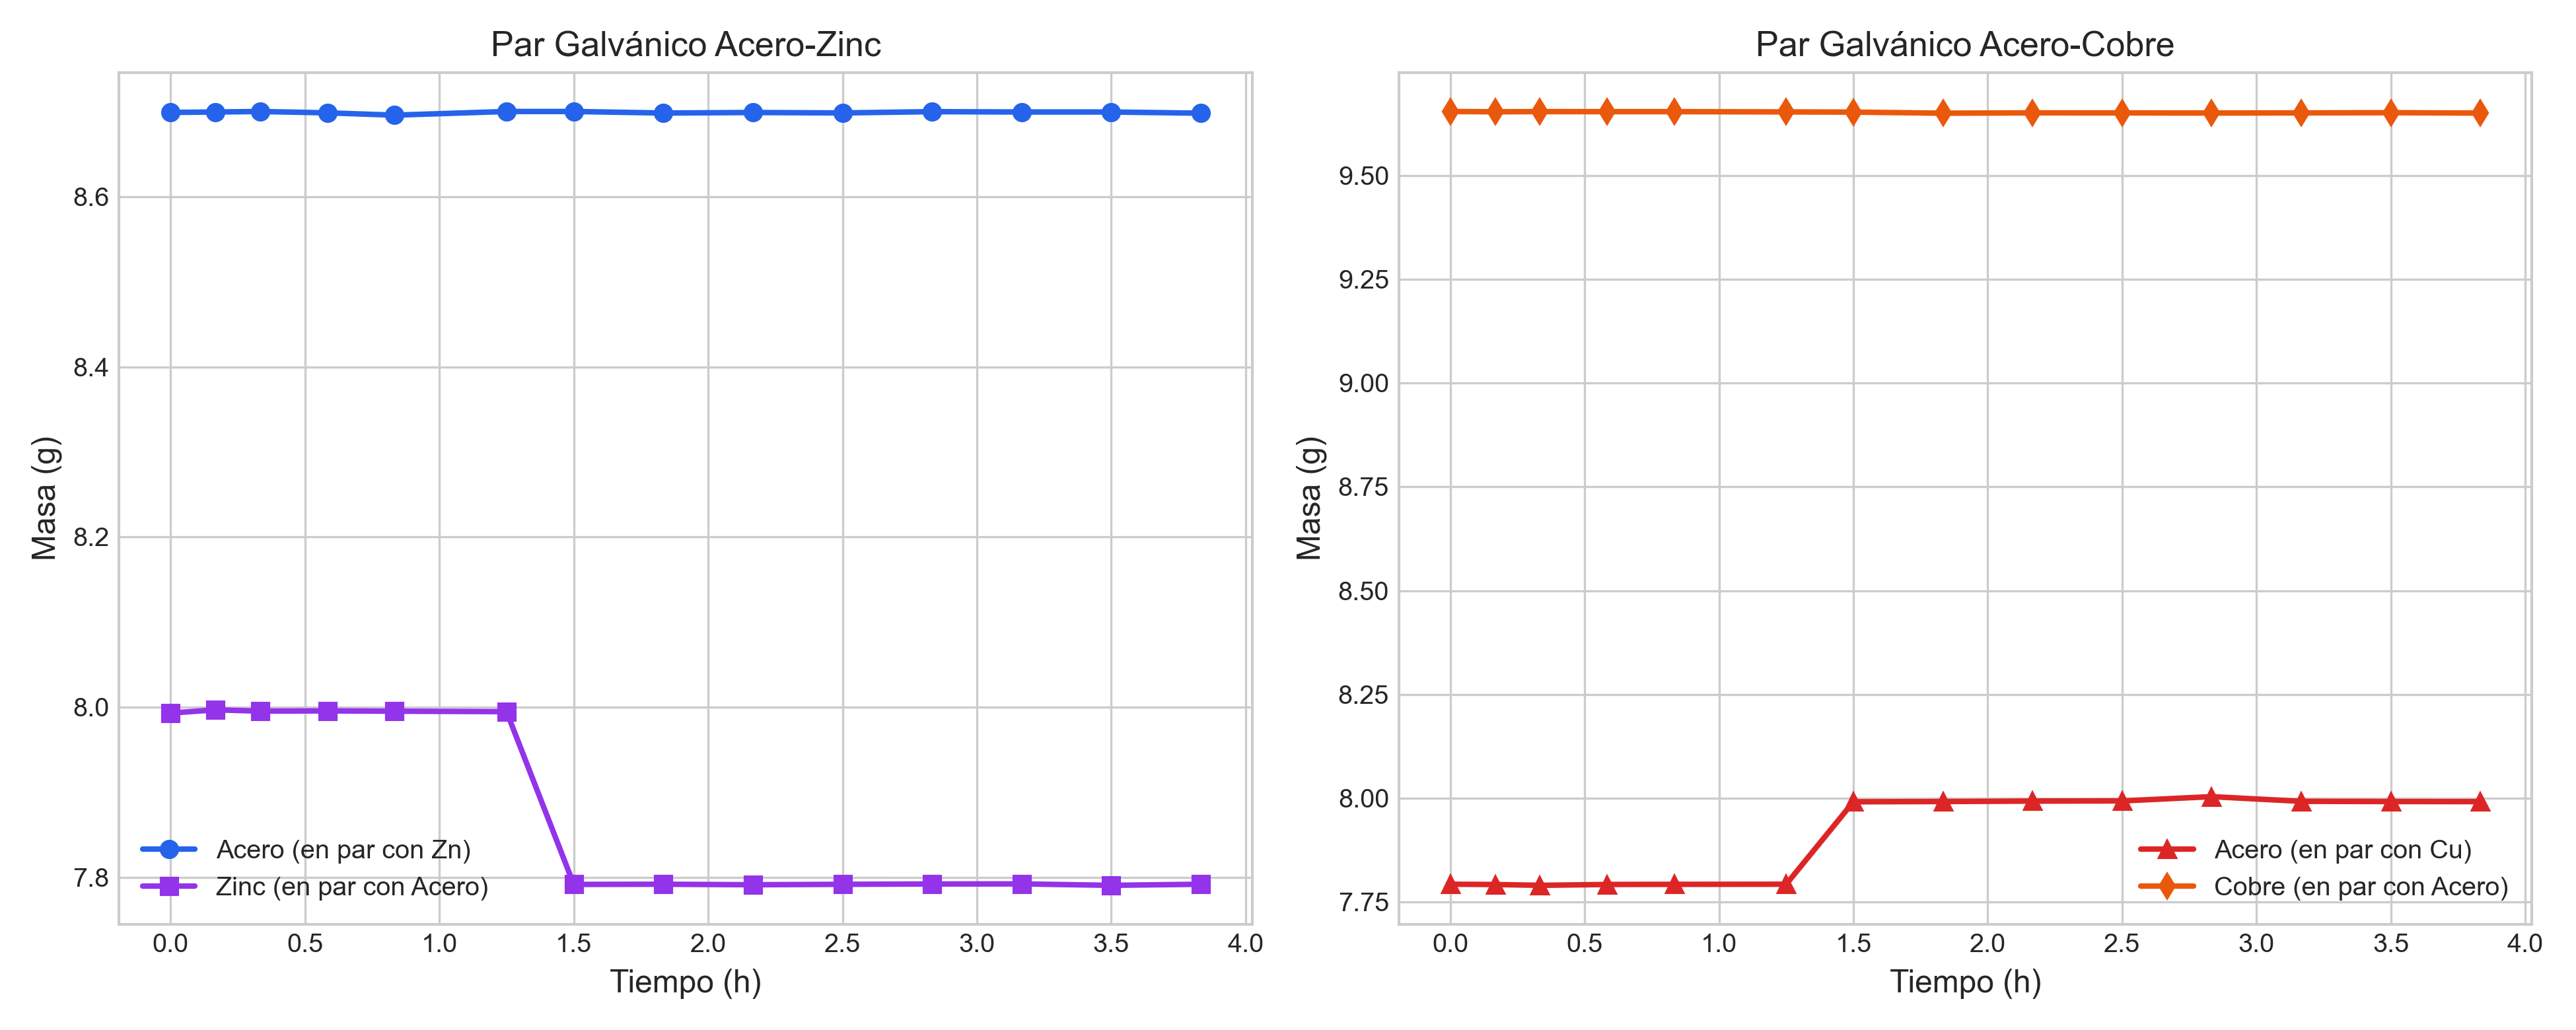
\includegraphics[width=0.92\textwidth]{resultados_practica_corrosion/exp_3_6_masa.png}
    \caption{Evolución de masa para los pares galvánicos Acero-Zn y Acero-Cu.}
    \label{fig:exp_3_6_masa}
\end{figure}

\begin{figure}[H]
    \centering
    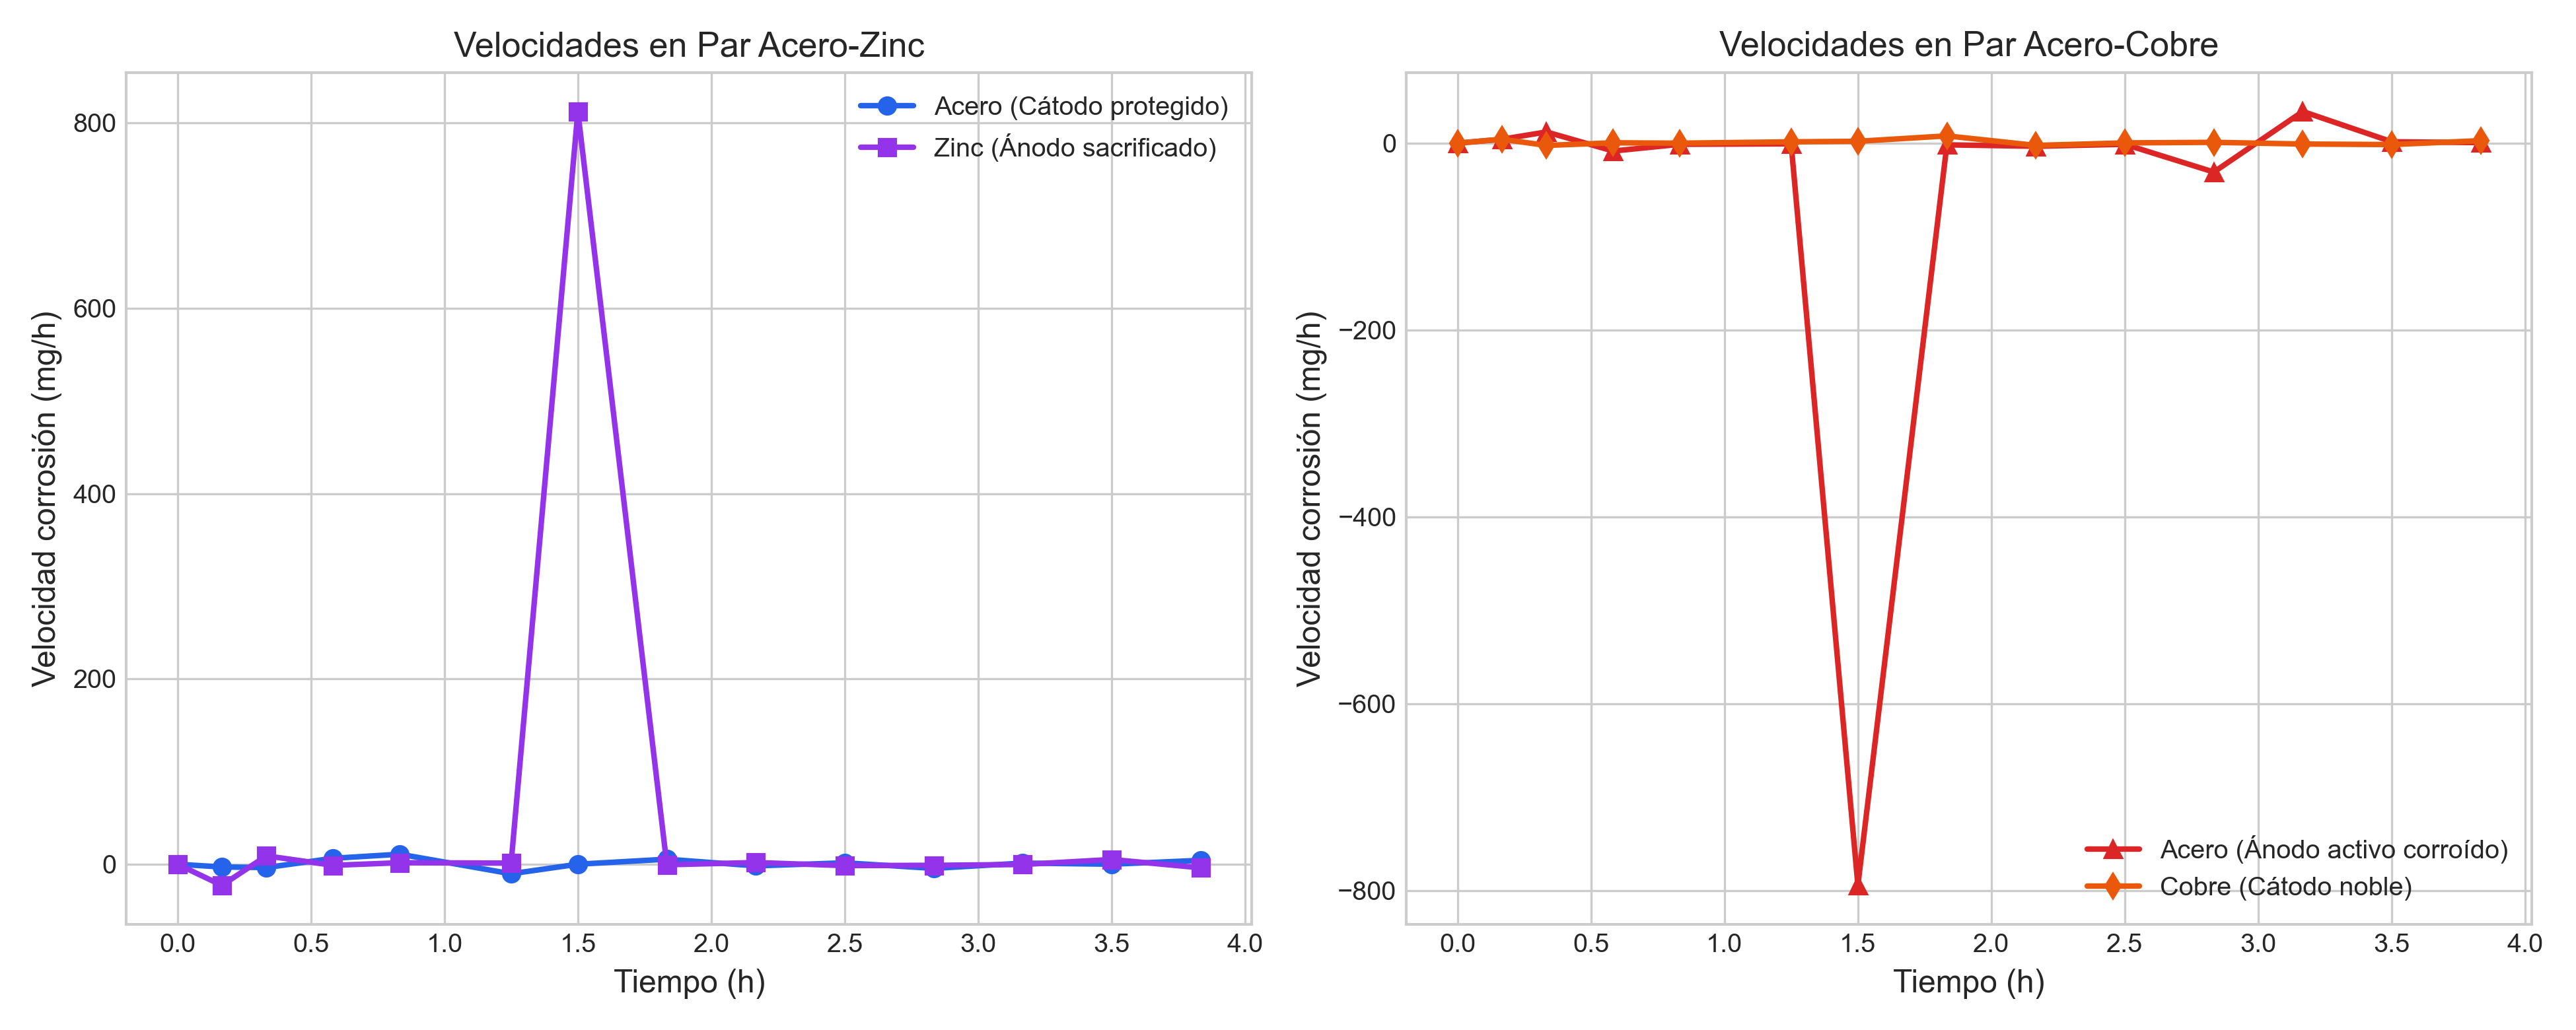
\includegraphics[width=0.92\textwidth]{resultados_practica_corrosion/exp_3_6_velocidad_corrosion.png}
    \caption{Velocidades de corrosión de los metales acoplados galvánicamente.}
    \label{fig:exp_3_6_vel}
\end{figure}

% =============================================================================
\section{Discusión Global y Conclusiones Generales}
% =============================================================================
A partir de los resultados experimentales obtenidos en las seis actividades de laboratorio, se extraen las siguientes conclusiones fundamentales para la ingeniería química y el diseño mecánico:

\begin{enumerate}
    \item \textbf{Efecto del pH y Termodinámica de Pourbaix (Exp. 3.1)}:
    El pH del medio determina la estabilidad termodinámica de las fases metálicas y sus óxidos. El zinc sufre corrosión severa en medio ácido ($v > 1.2\text{ mg/h}$) por inestabilidad de especies oxidadas solubles ($\text{Zn}^{2+}$), mientras que en medio básico entra en la zona de pasivación formando $\text{Zn(OH)}_2$, reduciendo su velocidad en más de un orden de magnitud. El cobre, al poseer potencial estándar noble (+0.34 V), requiere oxígeno disuelto para su ataque y presenta una resistencia muy superior.

    \item \textbf{Sensibilidad a Tensiones Residuales y Concentración de Esfuerzos (Exp. 3.2)}:
    Las zonas sometidas a deformación plástica o discontinuidades geométricas (taladros, entallas) actúan como microánodos galvánicos debido al incremento de energía libre local. Esto demuestra la necesidad crítica de realizar tratamientos térmicos de recocido de alivio de tensiones y diseñar transiciones geométricas suaves en recipientes a presión y tuberías.

    \item \textbf{Papel del Oxígeno como Despolarizante Catódico (Exp. 3.3)}:
    En electrolitos neutros, la velocidad de corrosión está controlada por la velocidad de difusión del oxígeno disuelto hacia el cátodo. La eliminación de oxígeno mediante ebullición o secuestradores químicos (como sulfito sódico o hidracina en calderas) detiene prácticamente la corrosión del acero.

    \item \textbf{Acción Protectora de Inhibidores Químicos Anódicos (Exp. 3.4)}:
    El fosfato trisódico ($\text{Na}_3\text{PO}_4$) precipita fosfato ferroso insoluble en las zonas anódicas, bloqueando la disolución metálica a concentraciones suficientes ($40\text{ mg/L}$). Se concluye que dosis bajas ($2\text{ mg/L}$) son contraproducentes si no aseguran la pasivación completa, ya que pueden derivar en corrosión localizada por picaduras.

    \item \textbf{Eficacia de la Protección Catódica por Corriente Impresa (Exp. 3.5)}:
    La polarización catódica forzada desplaza el potencial del acero a la región de inmunidad, evitando la oxidación del metal y concentrando la reacción catódica en la reducción de agua a hidrógeno gaseoso ($\text{H}_2$). Este método es fundamental en tuberías enterradas, tanques de almacenamiento y estructuras marinas.

    \item \textbf{Compatibilidad de Materiales y Corrosión Galvánica (Exp. 3.6)}:
    El acoplamiento bimetálico obedece estrictamente a la serie galvánica. El zinc protege sacrificialmente al acero (principio del galvanizado), mientras que el cobre acelera dramáticamente la corrosión del acero. En diseño industrial, debe evitarse el contacto directo entre metales dispares o intercalar juntas dieléctricas aislantes.
\end{enumerate}

\end{document}
